\documentclass{mcmthesis}
\mcmsetup{CTeX = True,   % 使用 CTeX 套装时,设置为 true
        tcn = 2500387, problem = D,
        sheet = true, titleinsheet = true, keywordsinsheet = true,
        titlepage = false, abstract = false}
\usepackage{lipsum}
\usepackage{float}
\usepackage{graphicx}
\usepackage{indentfirst}
\usepackage[T1]{fontenc}
\usepackage{palatino}
\usepackage{tikz}
\usepackage{multirow}
\usepackage{xcolor}
\usepackage{cite}
\usepackage{pdfpages}
\usepackage{nicematrix}
\usepackage{enumitem}
\usepackage{algorithm,algorithmic}
\usepackage{subfigure,subcaption}
\usepackage{lastpage}
\usepackage[super]{natbib} 
\usepackage{tabularx} % 引入 tabularx 宏包
\usepackage{booktabs} % 用于美化表格
\usepackage{listings}%代码排版
\usepackage{subfigure}
\usepackage[dvipsnames,table,xcdraw]{xcolor}

\lstset{
    language=Python, % 设置语言
 basicstyle=\ttfamily, % 设置字体族
 breaklines=true, % 自动换行
 keywordstyle=\bfseries\color{NavyBlue}, % 设置关键字为粗体,颜色为 NavyBlue
 morekeywords={}, % 设置更多的关键字,用逗号分隔
 emph={self}, % 指定强调词,如果有多个,用逗号隔开
    emphstyle=\bfseries\color{Rhodamine}, % 强调词样式设置
    commentstyle=\itshape\color{black!50!white}, % 设置注释样式,斜体,浅灰色
    stringstyle=\bfseries\color{PineGreen!90!black}, % 设置字符串样式
    columns=flexible,
    numbers=left, % 显示行号在左边
    numbersep=2em, % 设置行号的具体位置
    numberstyle=\footnotesize, % 缩小行号
    frame=single, % 边框
    framesep=1em % 设置代码与边框的距离
}
\newcommand{\upcite}[1]{\textsuperscript{\textsuperscript{\cite{#1}}}} 
\title{After the Catastrophe: The Resilience of Baltimore}%标题
\begin{document}

\begin{abstract}

  The transportation network is closely related to the development of a city, influencing various aspects such as people's daily lives, the transportation efficiency of goods and commodities, and the city's economic development. The transportation network in Baltimore is severely affected by the aging infrastructure, posing potential safety hazards to the smooth operation of the network. In this paper, we construct a transportation network analysis model and propose spatially - adaptable optimization strategies.

    Firstly, our transportation network analyzes traffic by computing the importance of nodes. Since traditional algorithms often overlook the actual network conditions and merely focus on the topological structure, we have innovatively improved the traditional \textbf{K - Shell node importance evaluation algorithm}. We substitute the "degree" of nodes in the K - Shell algorithm with a combination of the weighted degree of nodes and the node's own weight. The node weight is mainly determined by the net passenger flow at the node, and the edge weight is determined by the average travel time of the road deduced from the \textbf{BPR} function. Considering that different stakeholders have diverse demands for the transportation network, we categorize them into three groups and investigate the GDP shares of different stakeholder groups, which renders the model we establish more comprehensive.
    
    For Problem 1, we apply the model to analyze the situation before and after the collapse of the Francis Scott Key Bridge. By comparing the changes in node importance before and after the bridge collapse, we find that the importance of the I - 895 tunnel, the I - 95 tunnel, and the inland detour routes has increased significantly. Additionally, we assess the impact of the bridge collapse on various stakeholders.
    
    For Problem 2, we first use the \textbf{K-Prototypes clustering algorithm} to cluster the data related to bus stops, and then we select one of the clusters for analysis. With the help of the node importance in the transportation network, the number of bus routes, and the passenger flow at bus stops, we believe that Baltimore should add the route shown as the red line in Figure \ref{fig:busroute}.
    
    For Problem 3, we first analyze the potential safety hazards of traffic congestion in the Baltimore transportation network. Then, based on \textbf{the LWR model} and the node importance scores, we determine the exponential growth model of traffic congestion. Finally, according to the characteristic that traffic congestion "grows exponentially in the early stage and slowly in the later stage", we formulate a congestion management strategy.
    
    Finally, we conduct a sensitivity analysis of the parameter $\alpha$ in the K - Shell algorithm to illustrate the robustness of the model.

\begin{keywords}
\textbf{Transportation Network; \, K - Shell; \, BPR; \, K - Prototypes; \, Baltimore}
\end{keywords}
\end{abstract}
\maketitle
%% Generate the Table of Contents, if it's needed.
%% \renewcommand{\contentsnamefont}{\normalfont\bfseries\fontfamily{<ebgaramond>}\selectfont}
\tableofcontents
\newpage

\section{Introduction}

\subsection{Problem Background}

\begin{figure}[H]
    \centering
    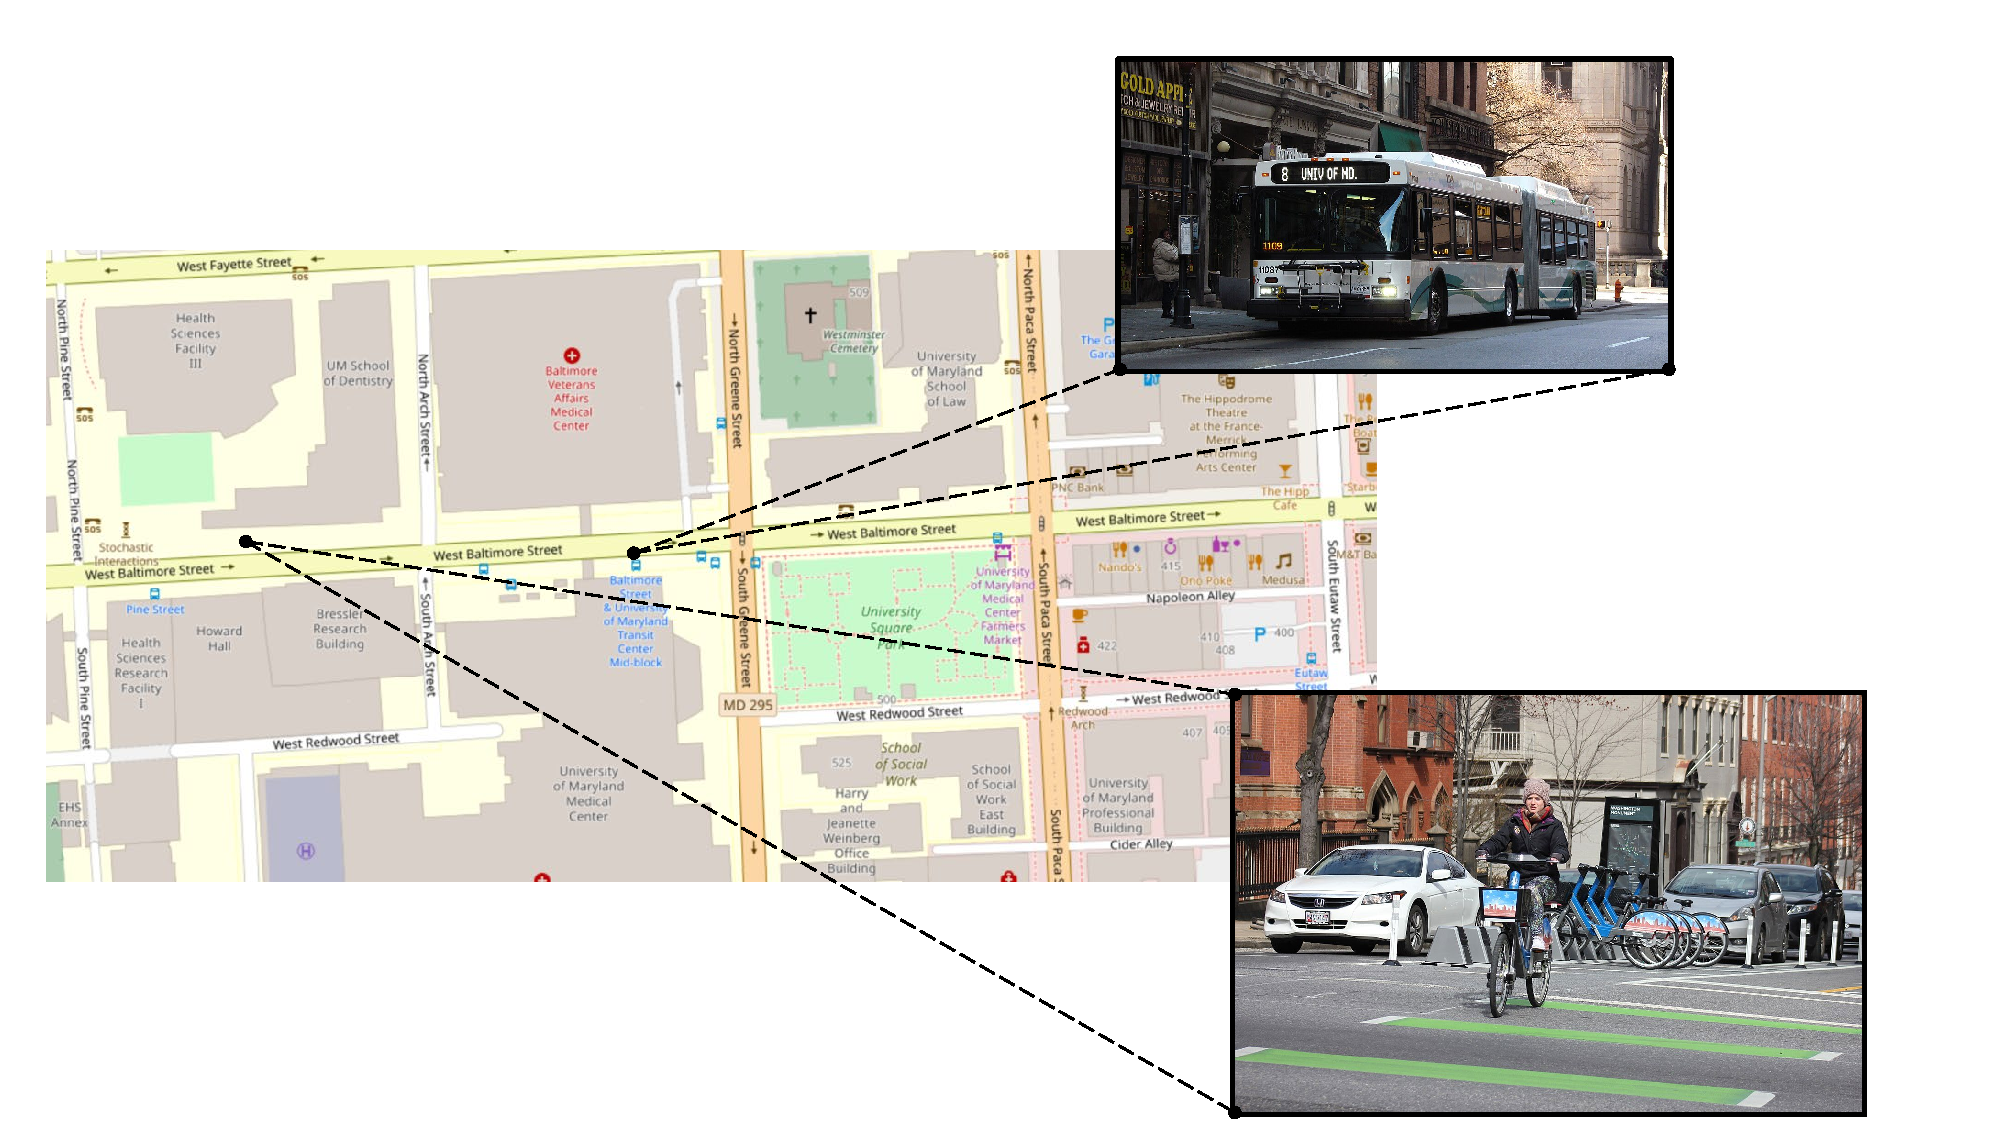
\includegraphics[width=\textwidth]{figures/intro.pdf}
    \caption{Various Transportation in Baltimore: Bicycles and Buses}
    \label{fig:intro}
\end{figure}

The transportation network is akin to the arteries of a city, which is crucial for a city's development and the living standards of its residents. This is also the case for Baltimore, Maryland, USA. Affected by the aging original infrastructure and limited transportation options, the Baltimore City Government is currently focusing on redesigning and optimizing its transportation system. The aim is to boost urban development, enhance the living standards and satisfaction of all stakeholders, while also adapting to future demands and ensuring sustainable development.

\subsection{Problem Restatement}
\label{sec:problem}

Based on the problem background information, we need to model the transportation network of Baltimore to improve the commuting experience of stakeholders. The main tasks are as follows:

\begin{enumerate}
  \item Based on the data provided in the problem, model and visualize the transportation network of Baltimore.
  \item Analyze the impact of the collapse of the Francis Scott Key Bridge on the transportation system in Baltimore and the impact on each stakeholder.
  \item Select a project that affects the bus system or the sidewalk system, analyze the impact of our Baltimore transportation network model on it, and analyze the impact on each stakeholder.
  \item Recommend a transportation network project that can best improve the lives of Baltimore residents and analyze it.
\end{enumerate}

\subsection{Literature Review}
\label{sec:zongshu}

According to the requirements put forward in section \ref{sec:problem}, we have searched a large number of literatures. The methods for analyzing key nodes in the network structure mainly include centrality methods based on the physical structure of the network \citep{ren2014}, degree - centrality algorithm \citep{zhang2017}, betweenness - centrality algorithm \citep{bergamini2014}, K - Shell algorithm \citep{maji2020}, PageRank algorithm \citep{tortosa2021}, etc. However, the above - mentioned methods only search for factors reflecting the importance of nodes from a single aspect, without considering the influence of various indicators in practical problems. They cannot fully explore the hidden characteristics of the network, so the accuracy of key - node identification results is relatively low. Based on these methods, this paper proposes an improved K - Shell decomposition algorithm based on node weights and edge weights and has achieved exciting results.

\begin{figure}[H]
  \centering
  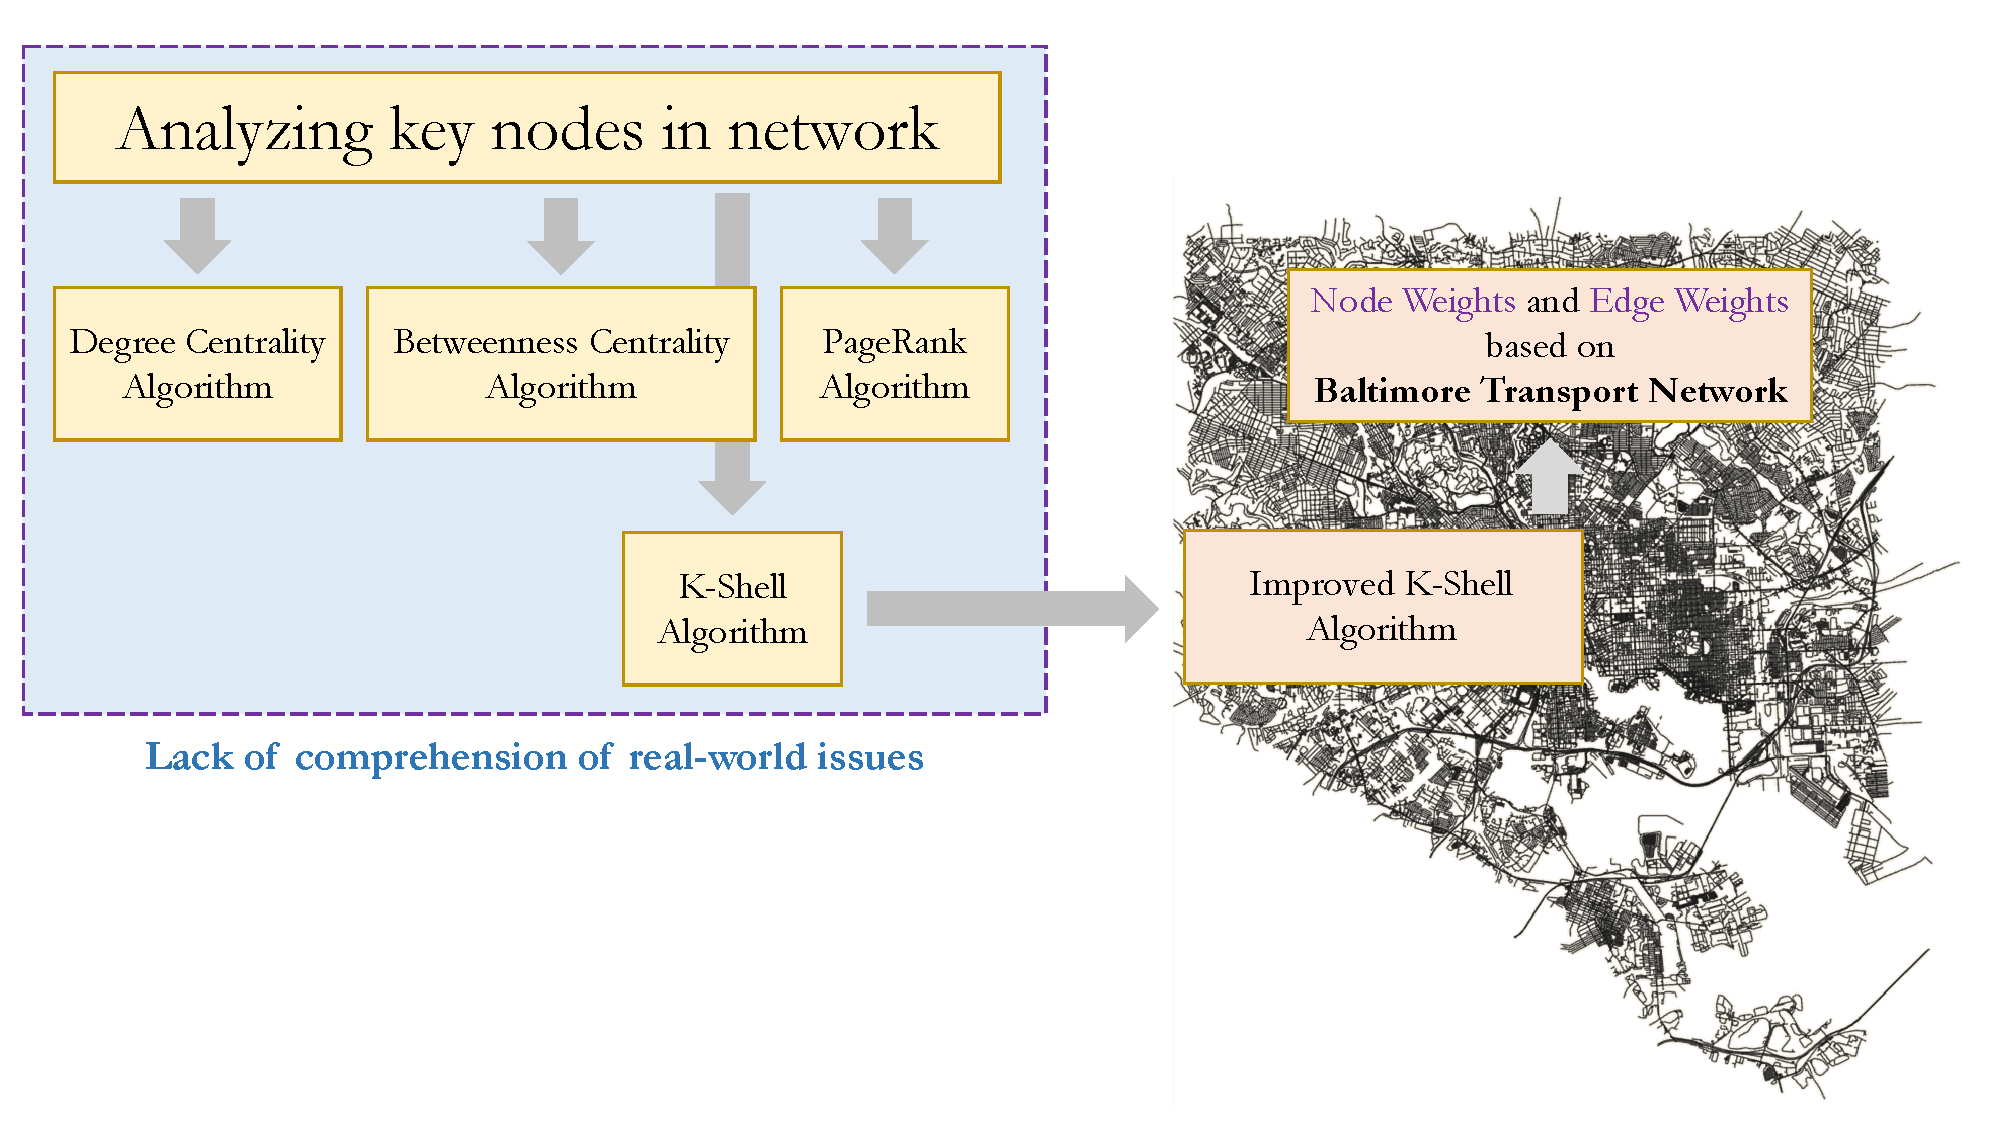
\includegraphics[width=\textwidth]{figures/zongshu.pdf}
  \caption{Thought Map of Literature Review}
  \label{fig:zongshu}
\end{figure}


\subsection{Our Work}

\begin{figure}[H]
  \centering
  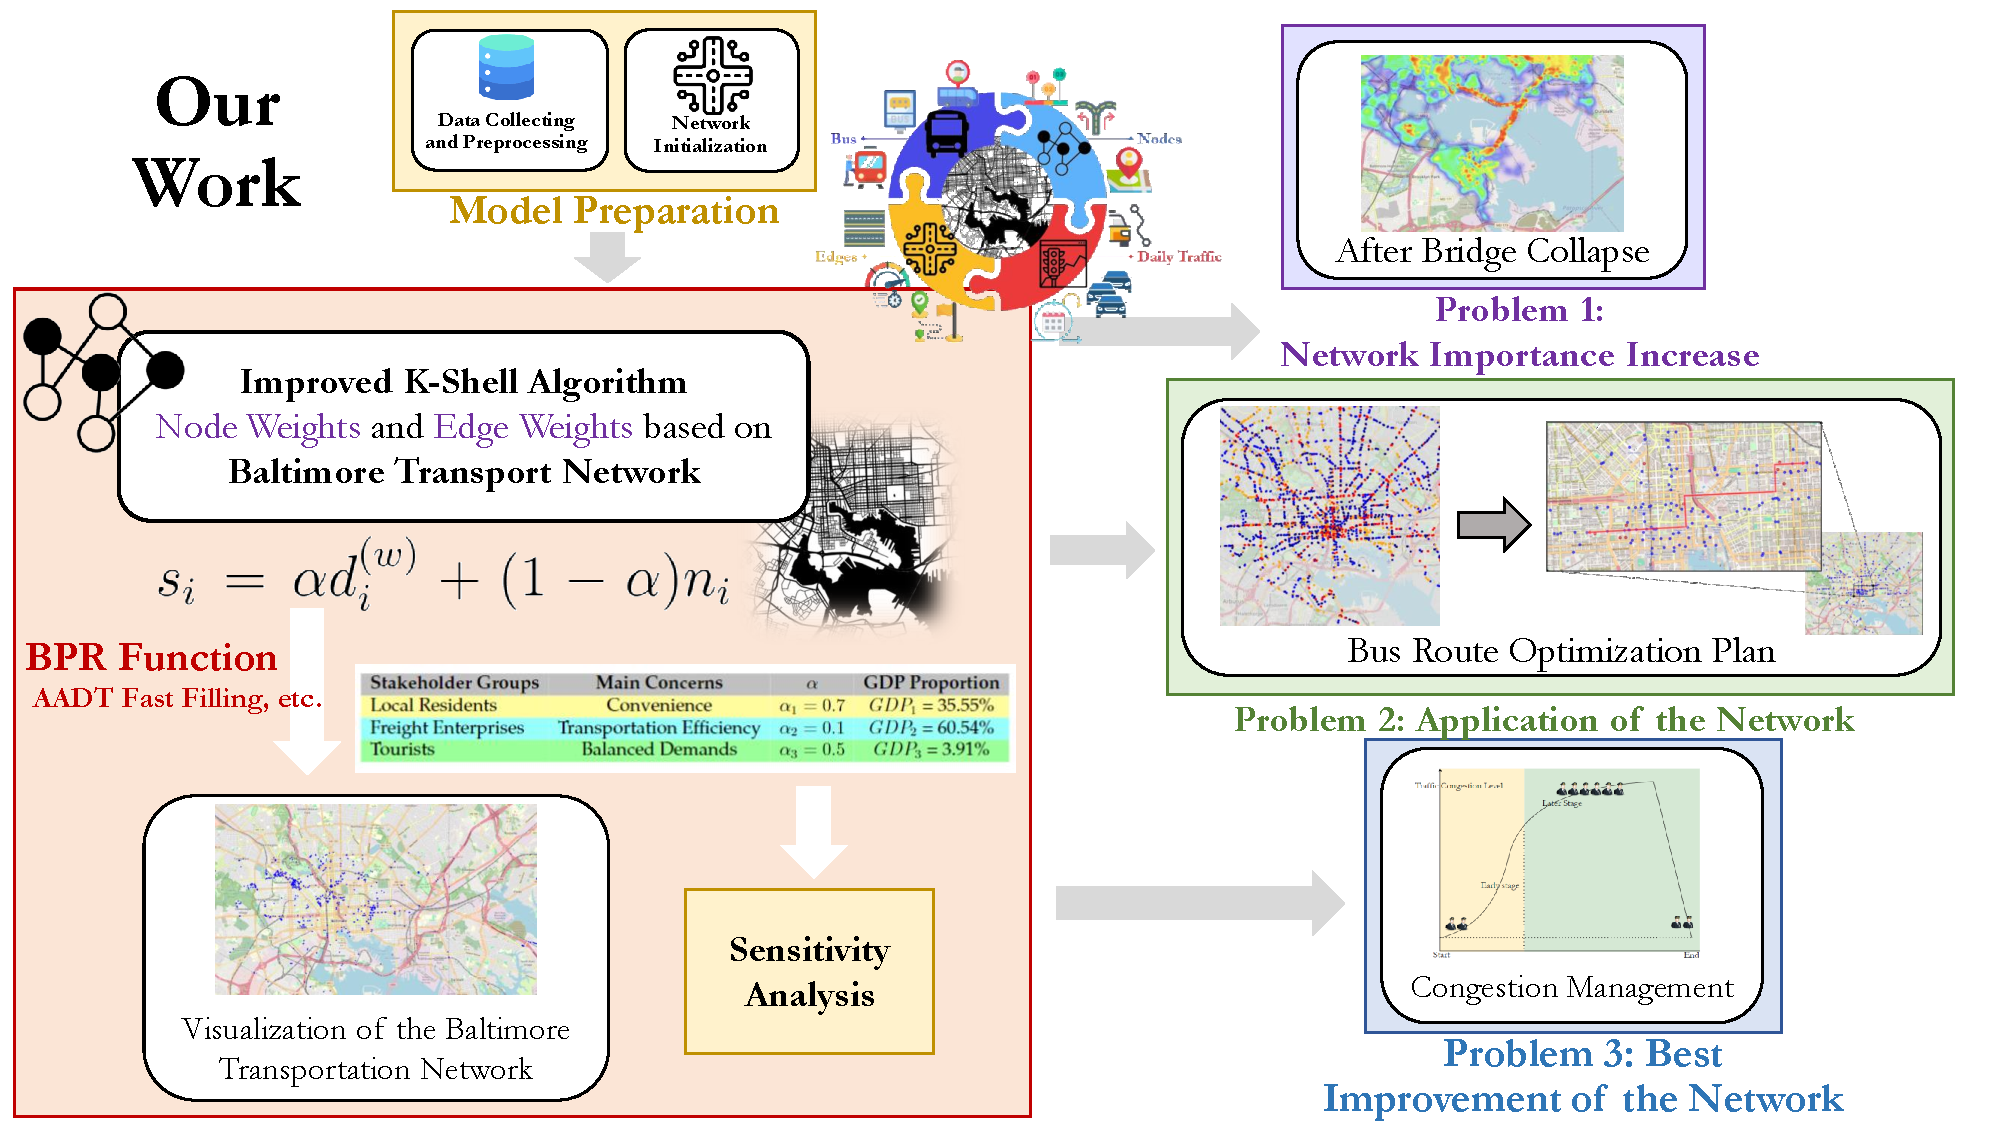
\includegraphics[width=\textwidth]{figures/ourwork.pdf}
  \caption{Our Work}
  \label{fig:ourwork}
\end{figure}

\section{Assumptions}

\begin{enumerate}
    \item Assume that the passenger flow at bus stops can, to a certain extent, reflect the nearby human flow, and after passengers get off, the passenger flow is evenly distributed on both sides of the road.
    \item Assume that the private road segments with \texttt{access=private} in the city of Baltimore do not belong to the urban transportation network.
    \item Assume that when considering the bus routes in Baltimore, \texttt{rider\_total} and \texttt{Stop\_Rider} in the dataset can fully represent the passenger flow.
\end{enumerate}

\section{Notation}

\begin{table}[H]
  \centering
  \caption{Symbols and Definitions}
  \label{tab:symbols}
  \begin{tabular}{cl}
    \toprule
    \textbf{Symbol}      & \textbf{Definition} \\
    \midrule
    $d_i^{(w)}$          & Weighted degree of node \\
    $n_i$                & Node weight \\
    $s_i$                & Node score \\
    $\alpha$             & Proportional coefficient of $d_i^{(w)}$ \\
    $\mathrm{score}$     & Evaluation score of the optimized bus route model \\
    $\rho(x,t)$          & Traffic density \\
    \bottomrule
  \end{tabular}
\end{table}

\section{Modeling of the Baltimore Transportation Network}

\subsection{Representation of the Network Model}

According to section \ref{sec:zongshu}, when traditional methods are used to build a transportation network model, most of them only rely on the topological structure of the network to analyze the importance of nodes, while ignoring important factors of the city such as passenger flow, climate, and terrain. However, we propose a K - Shell model based on node weights and edge weights. \textbf{The ratio of node weights and edge weights can represent the interests of all parties}, as shown in the table. This model not only takes into account the topological structure of the graph network but also the actual situation of the city. We abstract the urban transportation as a complex network \(G=(V, E)\), where \(|V| = N\), \(|E| = M\), and \(E\subseteq V\times V\).

The intersections or breakpoints of roads in the city are defined as nodes in the network \(G\), denoted as \(V=\{v_1, v_2, \ldots, v_N\}\), and the number of nodes is denoted as \(N\). All the roads in the city are defined as edges in the network \(G\), denoted as \(E = \{e_1, e_2, \ldots, e_M\}\), and the number of edges is denoted as \(M\).

\subsection{Improved K - Shell Decomposition Algorithm Based on Node and Edge Weights}
\label{sec:improvedKshell}

Given a directed graph \(G=(V, E)\) with node and edge weights, where \(V\) is the set of nodes and \(E\) is the set of edges. Each edge \(e_{ij}\in E\) has a weight \(w_{ij}\), and each node \(v_i\in V\) has a weight \(n_i\).

\subsubsection{Classification of Known Data}

\begin{figure}[H]
  \centering
  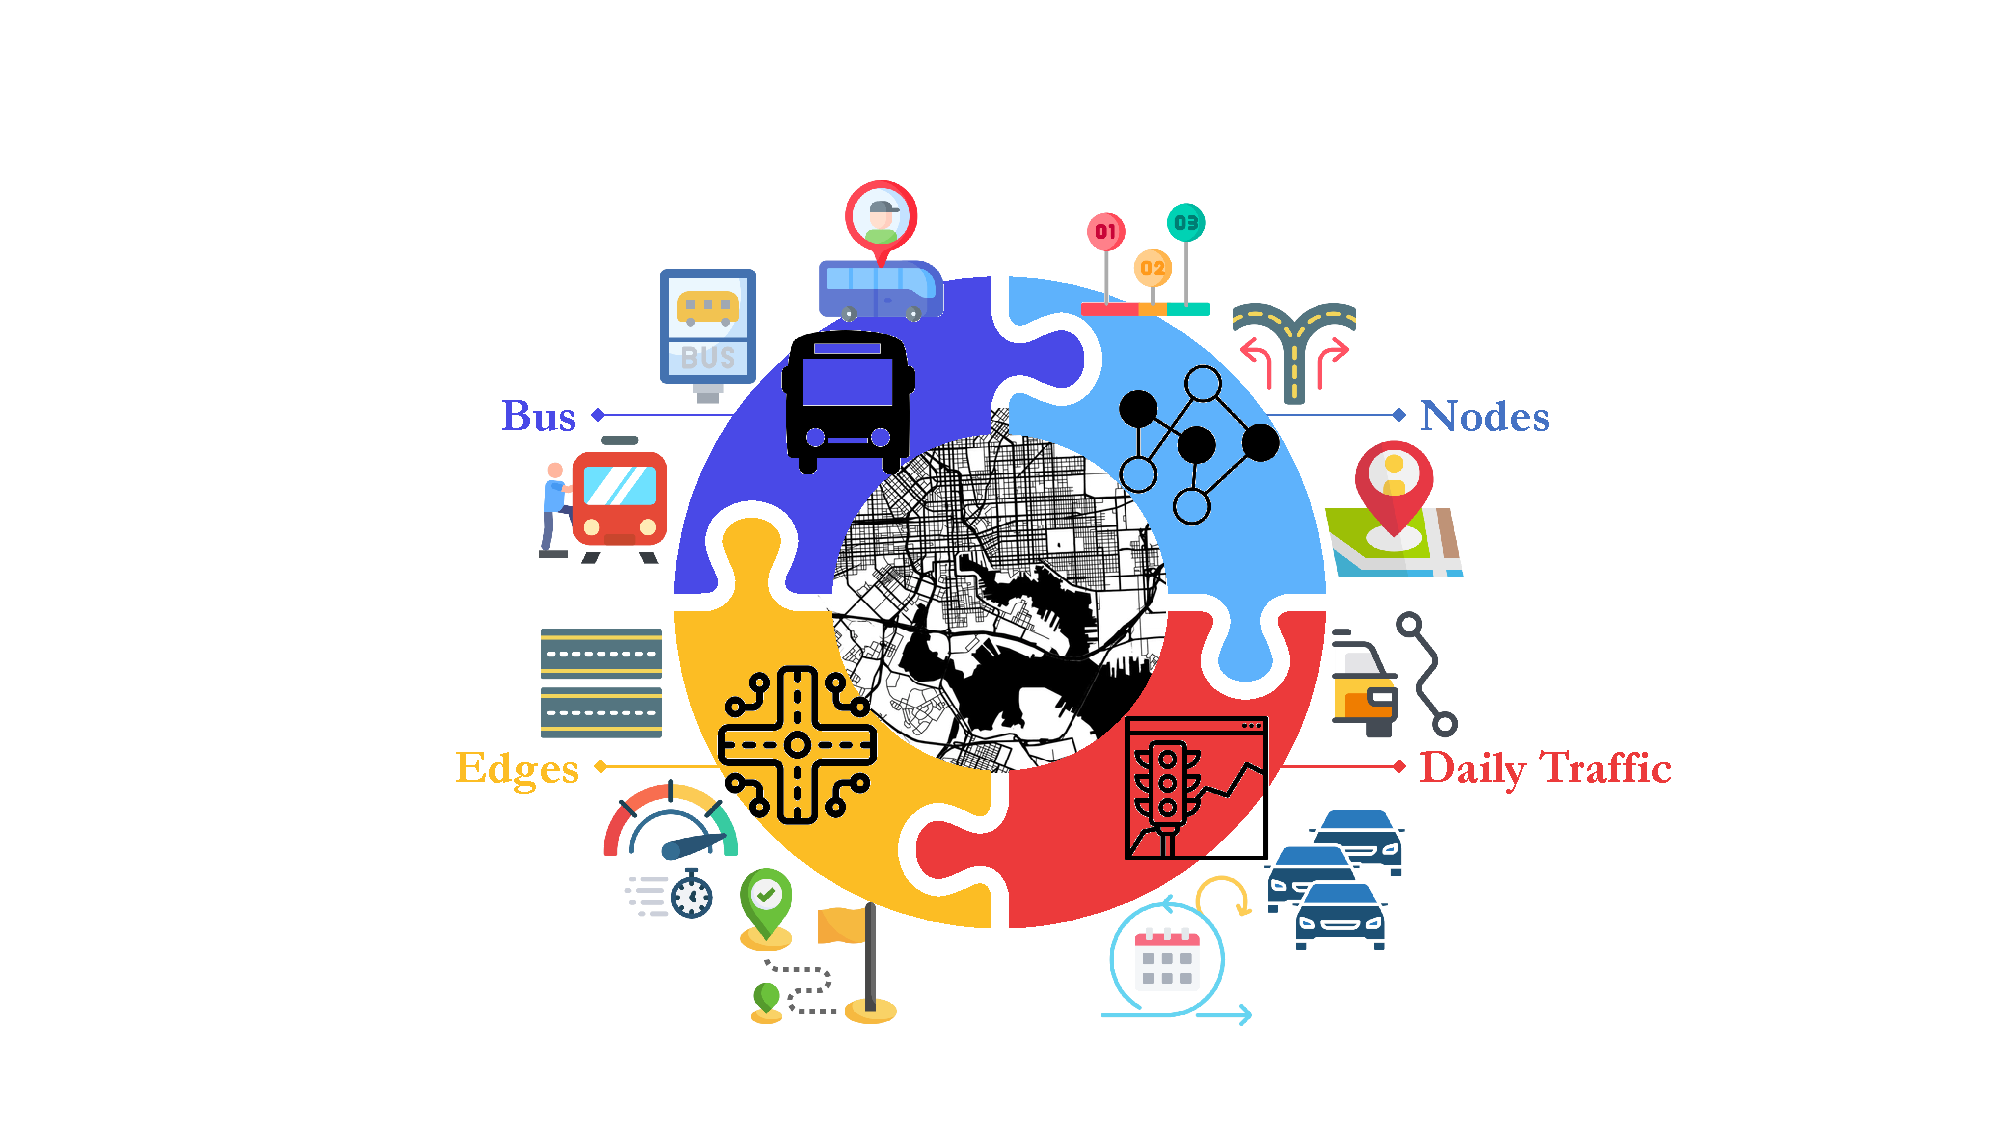
\includegraphics[width=0.8\textwidth]{figures/data.pdf}
  \caption{Types of Known Data}
  \label{fig:data}
\end{figure}

We can divide the Baltimore data items into two categories. One category describes the road network and intersections, and the other describes traffic flow and its fluctuations. Some of these items are related to node weights, and some are related to edge weights. The division is as follows:

Data for calculating node weights comes, on the one hand, from nodes, such as their longitude and latitude positions \texttt{X} and \texttt{Y}, the number of streets connected to the node \texttt{street\_count}, the intersection type \texttt{junction}, etc. On the other hand, it comes from data of bus stops, such as the position of the stop \texttt{X} and \texttt{Y}, the total number of passengers getting on and off at the stop \texttt{Rider\_Tota}, the total cumulative number of passengers at the stop \texttt{Stop\_Rider}, etc.

Data for calculating edge weights mainly comes from edges, such as their start and end points \texttt{u} and \texttt{v}, the number of lanes \texttt{lanes}, the maximum speed \texttt{maxspeed}, the length \texttt{length}, the service type \texttt{service}, etc. There is also some data from various traffic volumes, such as the ridership of bus routes \texttt{Distributi}, \texttt{AAWDT}, \texttt{AVMT}, \texttt{AADT}, etc. Finally, the flow direction of vehicles is also very important, such as the directional flow adjustment coefficient \texttt{D - Factor}, the peak - hour traffic volume adjustment coefficient \texttt{K - Factor}, etc.

\subsubsection{Improved K - Shell Decomposition Algorithm}

\begin{table}[H]
  \centering
  \label{tab:improvedKshell}
  \begin{tabular}{@{}p{0.95\textwidth}@{}}
  \toprule
  \textbf{Algorithm 1: The Improved K - Shell Decomposition Algorithm for Key Node Identification} \\ 
  \midrule
  \textbf{Input:} Graph network \(G=(V, E)\) \\
  \textbf{Output:} Node importance ranking result \\
  \textbf{Step 1:} Calculate the initial weighted degree of each node \(d_i^{(w)}=\sum_{j\in N(i)}w_{ij}\), where \(N(i)\) represents the set of adjacent nodes of node \(i\). \\
  \textbf{Step 2:} For each node \(i\), calculate the score \(s_i\) given by a certain stakeholder using the formula \(s_i=\alpha d_i^{(w)}+(1 - \alpha)n_i\). \textbf{Here, \(\alpha\) is a regulatory parameter, which can reflect the priority requirements of different stakeholders for node weights and edge weights in the transportation network. See section \ref{sec:alpha}.} Both \(d_i^{(w)}\) and \(n_i\) are normalized using the min - max normalization method. \\
  \textbf{Step 3:} Iteratively remove nodes with low scores
  \begin{itemize}
      \item Find the set \(S\) of nodes with the lowest comprehensive scores in the current graph.
      \item Assign these nodes to the current K - Shell layer and remove them from the graph.
      \item Update the weighted degrees of the remaining nodes:
      \begin{equation}
          d_j^{(w)}=d_j^{(w)}-w_{ij}\quad\text{for all }j\in N(i)
      \end{equation}
  \end{itemize}
  \textbf{Step 4:} Repeat the above steps for the remaining graph until all nodes are assigned to a certain K - Shell layer. \\ \bottomrule
  \end{tabular}
\end{table}

\subsection{Determination of Node and Edge Weights}

\subsubsection{Determination of Node Weight}

The node weight mainly considers the government's perspective. When the human flow at a certain node increases, it can promote local economic development, boost tourism, and increase the vitality of enterprises. Therefore, we use the net flow of the node as the standard for the node weight.

According to Assumption 1, the directions of passengers getting on and off are evenly distributed. We have:

\begin{itemize}
  \item Passengers getting on the bus enter the road from nodes \(u\) and \(v\) at a ratio of \(\frac{U_{uv}}{2}\), where \(U_{uv}\) represents the total number of passengers entering the road at this stop.
  \item Passengers getting off the bus head towards nodes \(u\) and \(v\) at a ratio of \(\frac{D_{uv}}{2}\), where \(D_{uv}\) represents the total number of passengers leaving the road at this stop.
\end{itemize}

We define the set of adjacent edges of a certain node \(u\) as \(\mathcal{E}\). First, calculate the outflow (passengers leaving the node) and inflow (passengers arriving at the node) of the node:

\begin{equation}
  \begin{cases} 
  \text{Outflow}(i)=\dfrac{1}{2}\sum_{(i, j)\in\mathcal{E}}U_{ij} \\
  \text{Inflow}(i)=\dfrac{1}{2}\sum_{(j, i)\in\mathcal{E}}D_{ji} 
  \end{cases}
\end{equation}

Finally, we calculate the net flow of the node to represent the node weight:

\begin{equation}
\text{Net}(i)=\text{Inflow}(i)-\text{Outflow}(i)=\frac{1}{2}\sum_{(i, j)\in\mathcal{E}}U_{ij}-\frac{1}{2}\sum_{(j, i)\in\mathcal{E}}D_{ji}
\end{equation}

\subsubsection{Determination of Edge Weight}

The edge weight is mainly measured by the travel time of local residents, tourists, and transit passengers. We collect indicators related to the edge weight from the data file, such as road type, the number of lanes on the road segment, the maximum speed limit on the road, whether the road is one - way, road length, road width, and the number of lanes. Based on these, we establish the following model:

The BPR function describes the relationship between travel time and traffic flow:

\begin{equation}
t = t_0 \left(1 + \alpha \left(\frac{V}{C}\right)^\beta\right)
\end{equation}

where \(t\) represents the travel time, \(t_0\) is the free - flow time (travel time without congestion), \(V\) represents the traffic flow (e.g., AADT, Annual Average Daily Traffic), \(C\) represents the road capacity, and \(\alpha, \beta\) are empirical parameters (usually \(\alpha = 0.15\) and \(\beta = 4\)) \cite{hamdouch2014} \cite{gao2004}.

According to the BPR function, we can obtain the actual speed \(v\):

\begin{equation}
v = \frac{L}{t} = \frac{L}{t_0 \left(1 + \alpha \left(\frac{V}{C}\right)^\beta\right)},
\end{equation}

where \(L\) is the road length. Since the free - flow speed \(v_0=\frac{L}{t_0}\), we have:

\begin{equation}
v = \frac{v_0}{1 + \alpha \left(\frac{V}{C}\right)^\beta}.
\end{equation}

In addition, the road capacity \(C\) is affected by the number of lanes \texttt{lanes} and the road functional classification \texttt{Functional Class} (interstate highways, arterial roads, local roads). Finally, we introduce other adjustment factors:

\begin{itemize}
  \item Road feature correction
    \begin{itemize}
      \item Tunnel (\texttt{tunnel = yes}): The speed is reduced by 15\%, i.e., \(v_{\text{final}} = v\times0.85\).
      \item Bridge (\texttt{bridge = yes}): The speed is reduced by 10\%, i.e., \(v_{\text{final}} = v\times0.9\).
      \item One - way road (\texttt{oneway = True}): The speed is increased by 5\%, i.e., \(v_{\text{final}} = v\times1.05\).
    \end{itemize}
  \item Influence of the number of lanes
    \begin{itemize}
      \item The more lanes, the higher the traffic efficiency: \(C = C_{\text{base}}\times\text{lanes}\).
    \end{itemize}
\end{itemize}

After considering all factors, we can obtain:

\begin{equation}
v_{\text{final}} = \frac{v_0}{1 + \alpha \left(\frac{\text{AADT}}{C}\right)^\beta}\times f_{\text{tunnel}}\times f_{\text{bridge}}\times f_{\text{oneway}},
\end{equation}

where:

\begin{itemize}
  \item \(f_{\text{tunnel}} = 1 - 0.15\times\text{is\_tunnel}\), \(\text{is\_tunnel}\in\{0,1\}\)
  \item \(f_{\text{bridge}} = 1 - 0.1\times\text{is\_bridge}\), \(\text{is\_bridge}\in\{0,1\}\)
  \item \(f_{\text{oneway}} = 1 + 0.05\times\text{is\_oneway}\), \(\text{is\_oneway}\in\{0,1\}\)
\end{itemize}

Finally, the edge weight is determined by the travel time:

\begin{equation}
t=\frac{L}{v_{final}},
\end{equation}

where \(L\) represents the road length.

\subsection{Determination of \(\alpha\) by Stakeholders}
\label{sec:alpha}

After analyzing the situation in Baltimore, we divide the stakeholders into the following three main groups with different needs, and determine their \(\alpha\) values according to their work or life characteristics in section \ref{sec:source}, as shown in Table \ref{tab:stakeholder_data}:

% \begin{table}[H]
%   \centering
%   \caption{Stakeholder Data}
%   \label{tab:stakeholder_data}
%   \begin{tabular}{@{}lccc@{}}
%     \toprule
%     \textbf{Stakeholder Groups} & \textbf{Main Concerns} & \textbf{$\alpha$} & \textbf{GDP Proportion} \\
%     \midrule
%     Local Residents & Convenience & $\alpha_1 = 0.7$ & \(GDP_1\) = 35.55\%  \\
%     Freight Enterprises & Transportation Efficiency & $\alpha_2 = 0.1$ & \(GDP_2\) = 60.54\% \\
%     Tourists & Balanced Demands & $\alpha_3 = 0.5$ & \(GDP_3\) = 3.91\%  \\
%     \bottomrule
%   \end{tabular}
% \end{table}

\begin{table}[H]
  \centering
  \caption{Stakeholder Data}
  \label{tab:stakeholder_data}
  \begin{tabular}{@{}lccc@{}}
  \rowcolor[HTML]{C0C0C0} 
  \textbf{Stakeholder Groups} & \textbf{Main Concerns}    & \textbf{$\alpha$} & \textbf{GDP Proportion} \\
  \rowcolor[HTML]{FFFC9E} 
  Local Residents             & Convenience               & $\alpha_1 = 0.7$                   & \(GDP_1\) = 35.55\%                      \\
  \rowcolor[HTML]{96FFFB} 
  Freight Enterprises         & Transportation Efficiency & $\alpha_2 = 0.1$                   & \(GDP_2\) = 60.54\%                      \\
  \rowcolor[HTML]{9AFF99} 
  Tourists                    & Balanced Demands          & $\alpha_3 = 0.5$                   & \(GDP_3\) = 3.91\%                      
  \end{tabular}
\end{table}

Thus, we can establish the comprehensive network importance proportional coefficient for Baltimore:
\begin{equation}
  \alpha_{\text{total}}=\sum_{i = 1}^{n}\omega_i\cdot\alpha_i,\quad i = 1,2,3,
\end{equation}
where \(\omega_i\) is the weight of the stakeholder group, determined by the GDP proportion, i.e., \(\omega_i = GDP_i\).

After calculation, the final weight is:
\begin{equation}
  \alpha_{\text{total}}=0.32534
\end{equation}

\subsection{Data Preprocessing}

\subsubsection{Data Screening}

Since the geographical scope of the data provided in the problem is the Baltimore Metropolitan Area, which is much larger than the scope of Baltimore City, we first screen out the data within the scope of Baltimore City according to longitude and latitude. The screening results are shown in the following table:

\begin{table}[H]
  \centering
  \caption{Data Statistics Before and After Filtering}
  \label{tab:data_filtering_stats}
  \begin{tabular}{@{}lcc@{}}
      \toprule
      \textbf{Data Table} & \textbf{Before Filtering} & \textbf{After Filtering} \\
      \midrule
      edge\_all.csv & 565,495 entries & 201,003 entries \\
      edge\_drive.csv & 91,227 entries & 29,309 entries \\
      \bottomrule
  \end{tabular}
\end{table}

\subsubsection{Missing Value Filling: Fast - filling Algorithm to Determine AADT}

AADT data is only collected on roads with bus stops, while other roads lack such data. However, the time complexity of directly using the shortest - distance method to fill the missing AADT values is too high. Therefore, we use the following fast - filling algorithm to determine the AADT values of all roads.

\begin{table}[H]
  \centering
  \label{tab:AADTFilling}
  \begin{tabular}{@{}p{0.95\textwidth}@{}}
  \toprule
  \textbf{Algorithm 2: Fast Filling Algorithm for AADT Values of All Roads} \\ 
  \midrule
  \textbf{Step 1:} Assign the AADT value of all edges to 0, and update the AADT values of edges with bus stops. \\
  \textbf{Step 2:} Traverse the edges that have been assigned AADT values. For each such edge \(e_i\), traverse the edges \(e_j\) connected to it, and add the AADT value of \(e_i\) to the AADT list of \(e_j\). \\
  \textbf{Step 3:} Calculate the average value of the AADT list of \(e_j\) obtained in Step 2, and use it as the AADT value of \(e_j\). \\
  \textbf{Step 4:} Repeat Step 2 and Step 3 until there is no edge with an AADT value of 0 in the entire network. \\ \bottomrule
  \end{tabular}
\end{table}


\begin{figure}[H]
    \centering
    \subfigure[]{
    \begin{minipage}[t]{0.5\linewidth}
    \centering
    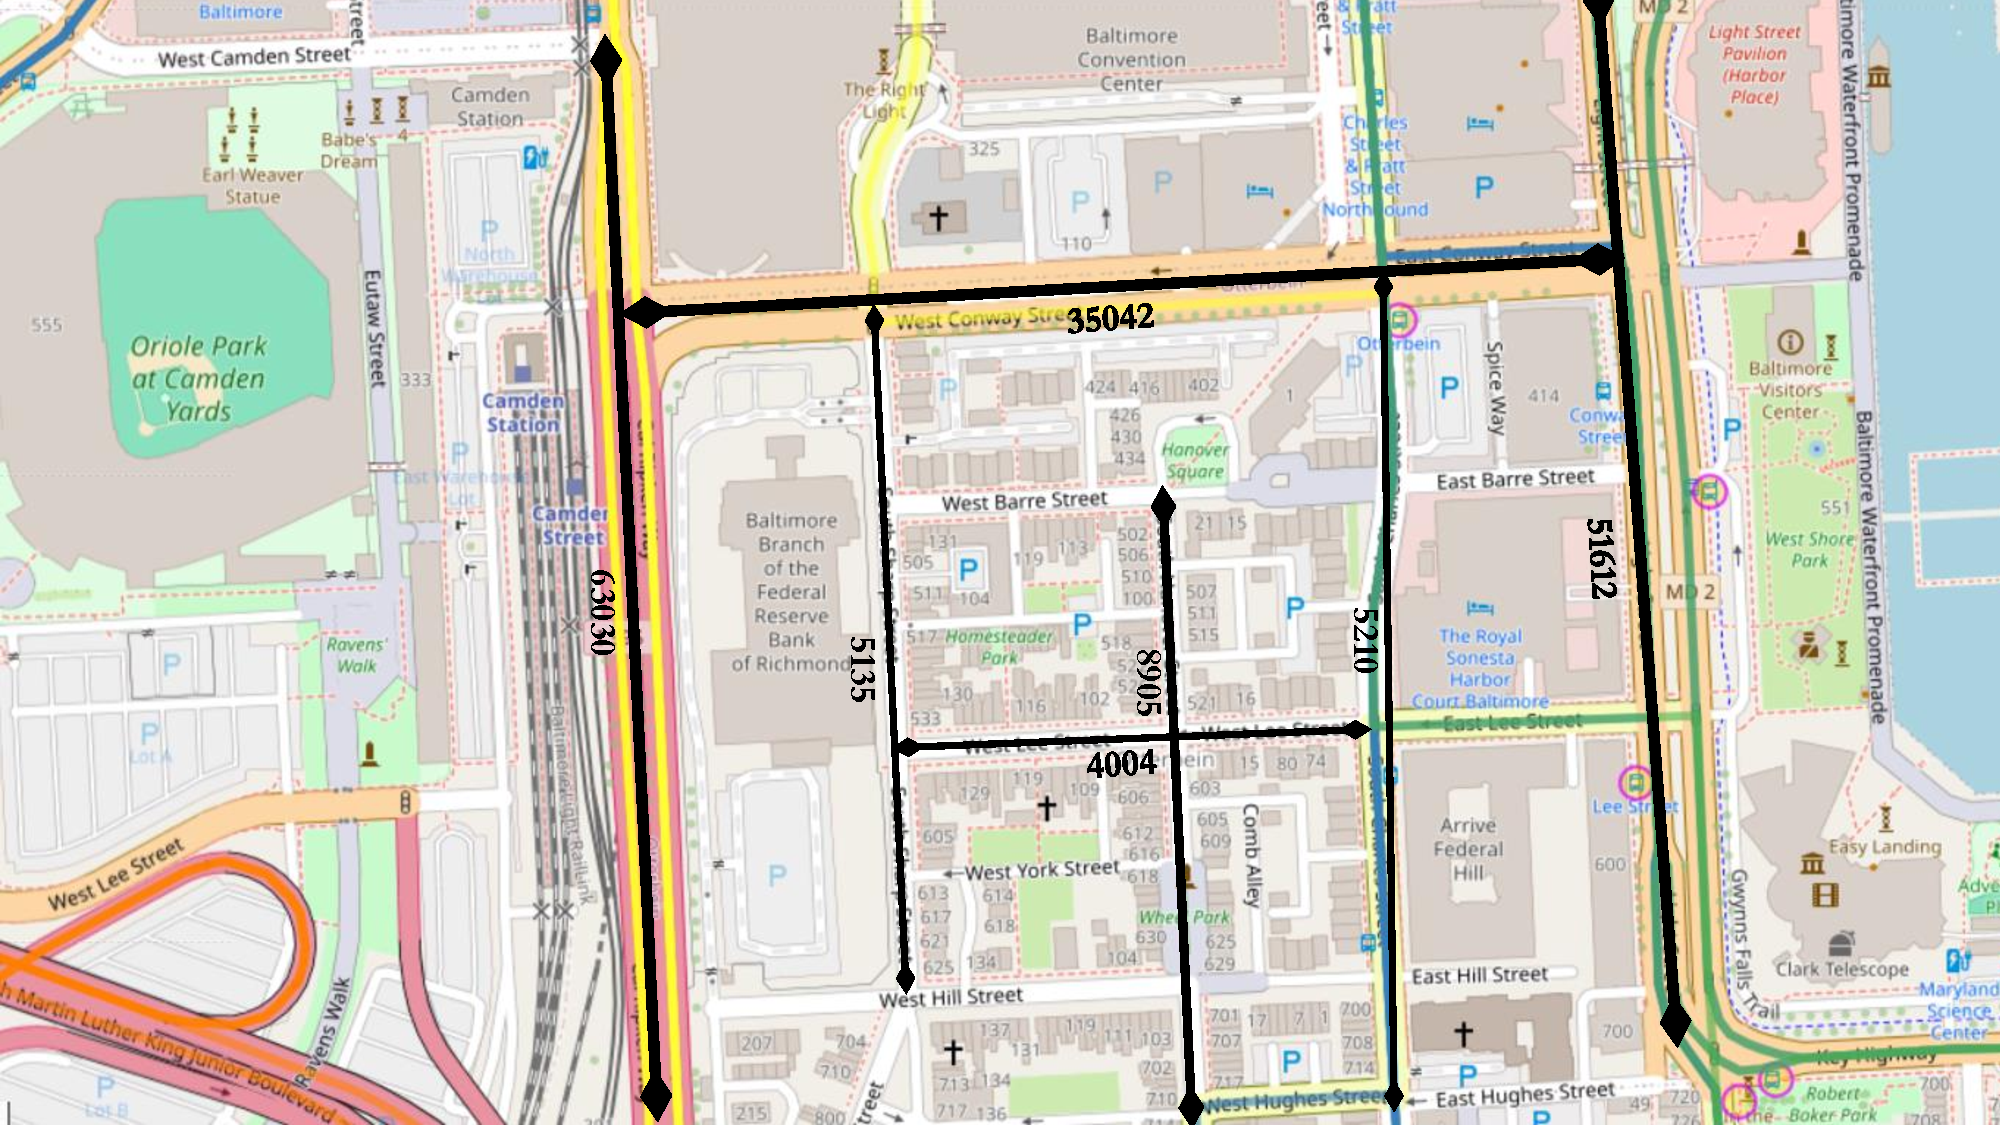
\includegraphics[width=\linewidth]{figures/topo1.pdf}
    \end{minipage}%
    % \label{fig:}%
    }%
    \subfigure[]{
    \begin{minipage}[t]{0.5\linewidth}
    \centering
    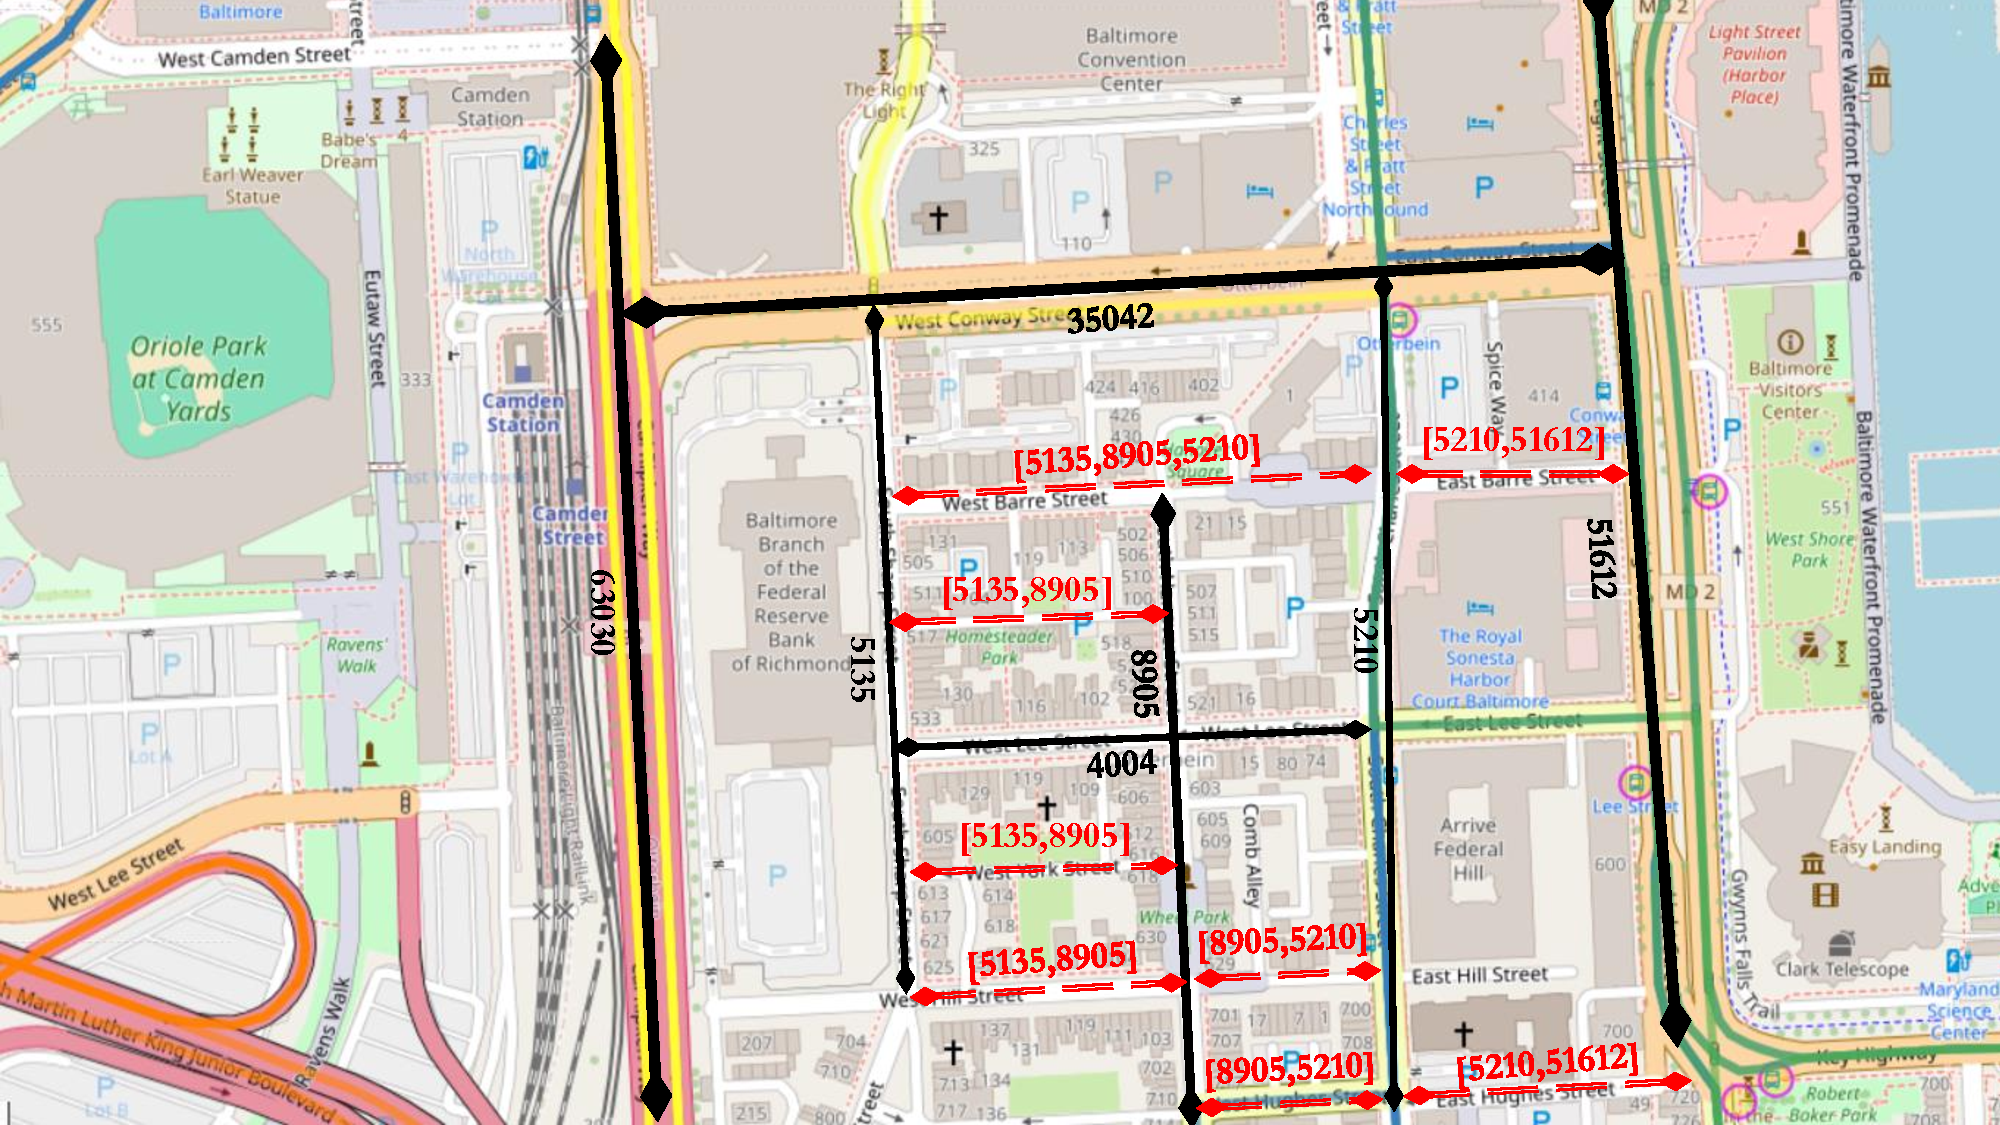
\includegraphics[width=\linewidth]{figures/topo2.pdf}
    \end{minipage}%
    % \label{fig:}%
    }%

    \subfigure[]{
        \begin{minipage}[t]{0.5\linewidth}
        \centering
        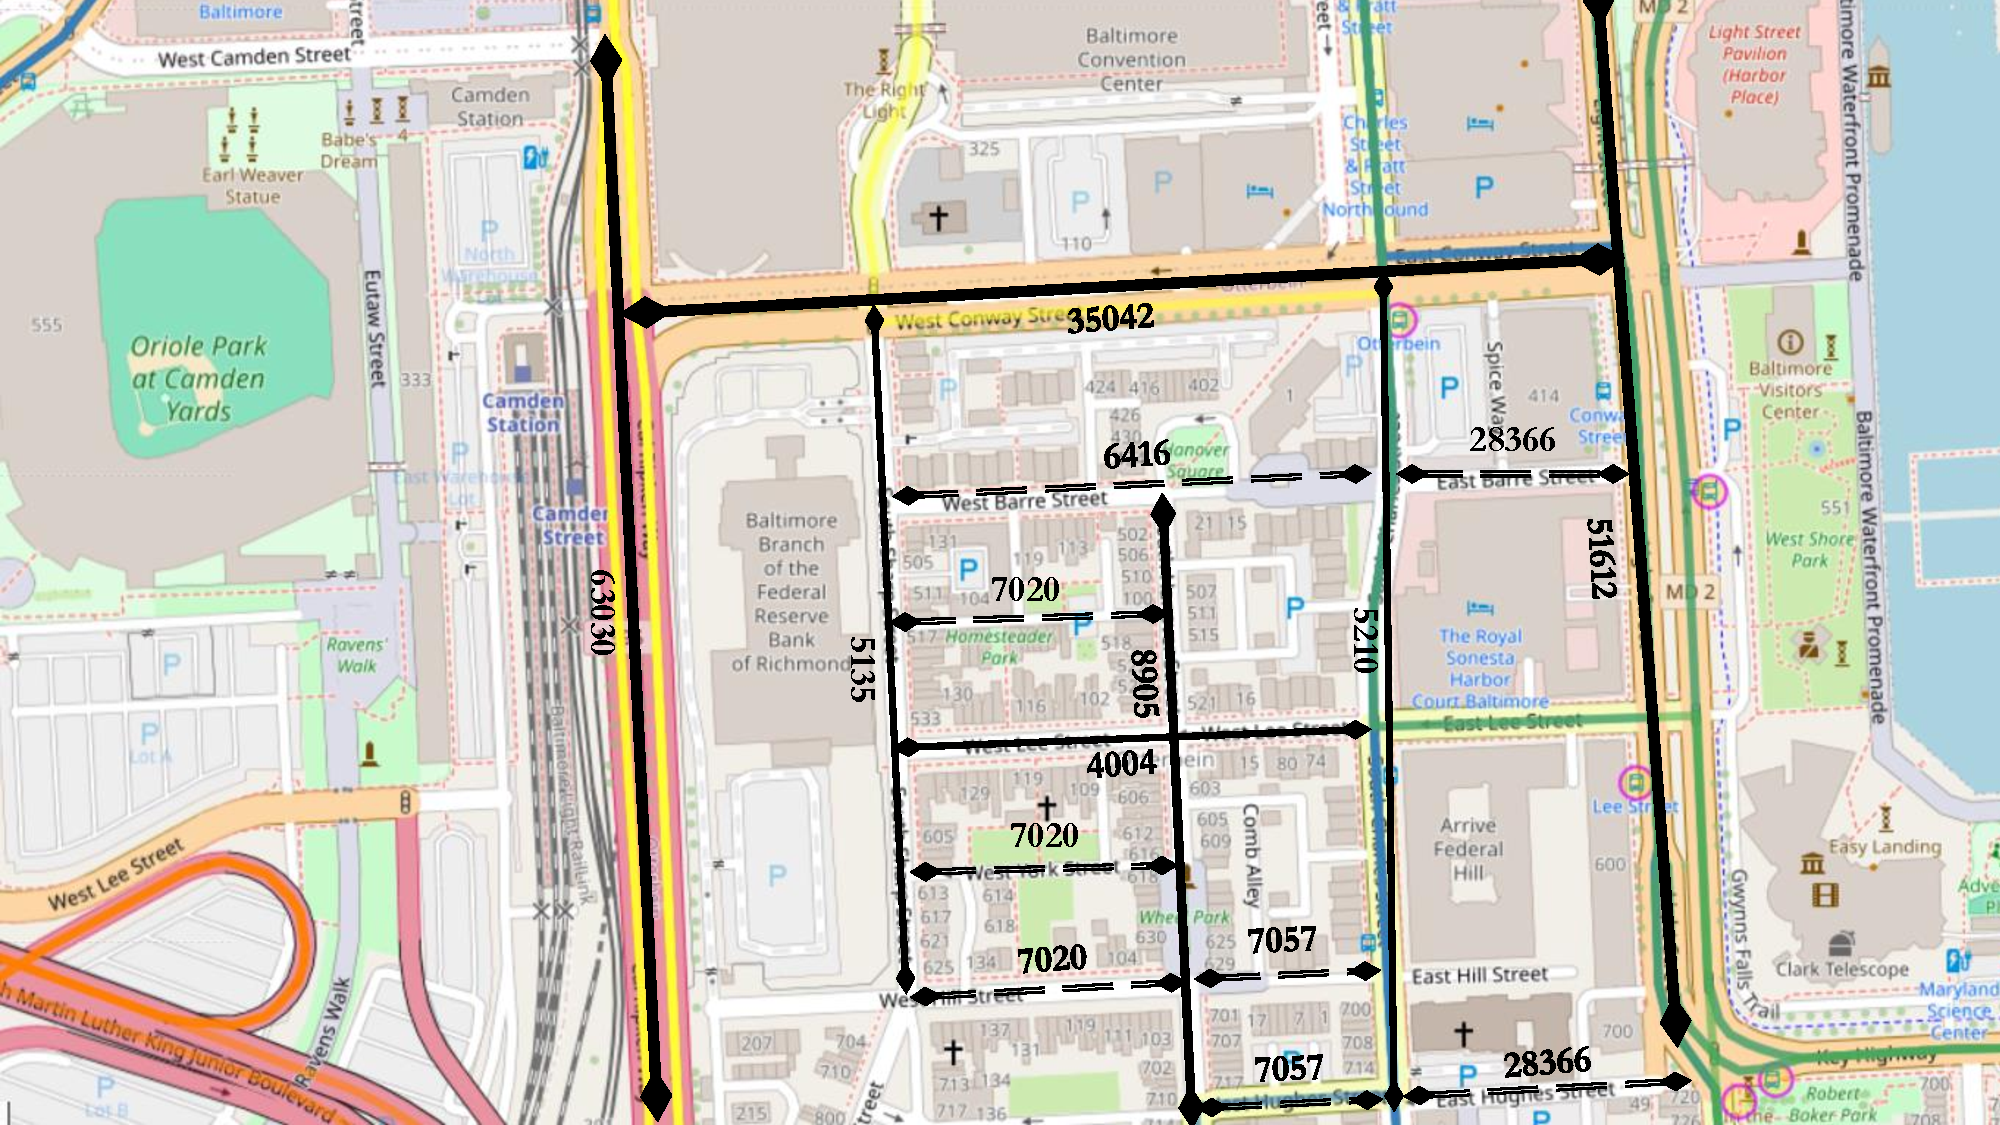
\includegraphics[width=\linewidth]{figures/topo3.pdf}
        \end{minipage}%
    % \label{fig:}%
    }%
    \caption{Example of AADT Filling}
    \label{fig:aadt}
\end{figure}

\subsection{Visualization of the Baltimore Transportation Network}

Based on the Baltimore urban transportation network model, we calculate the top 1000 nodes in terms of importance and visualize them. The results are shown in the figure below:

\begin{figure}[H]
  \centering
  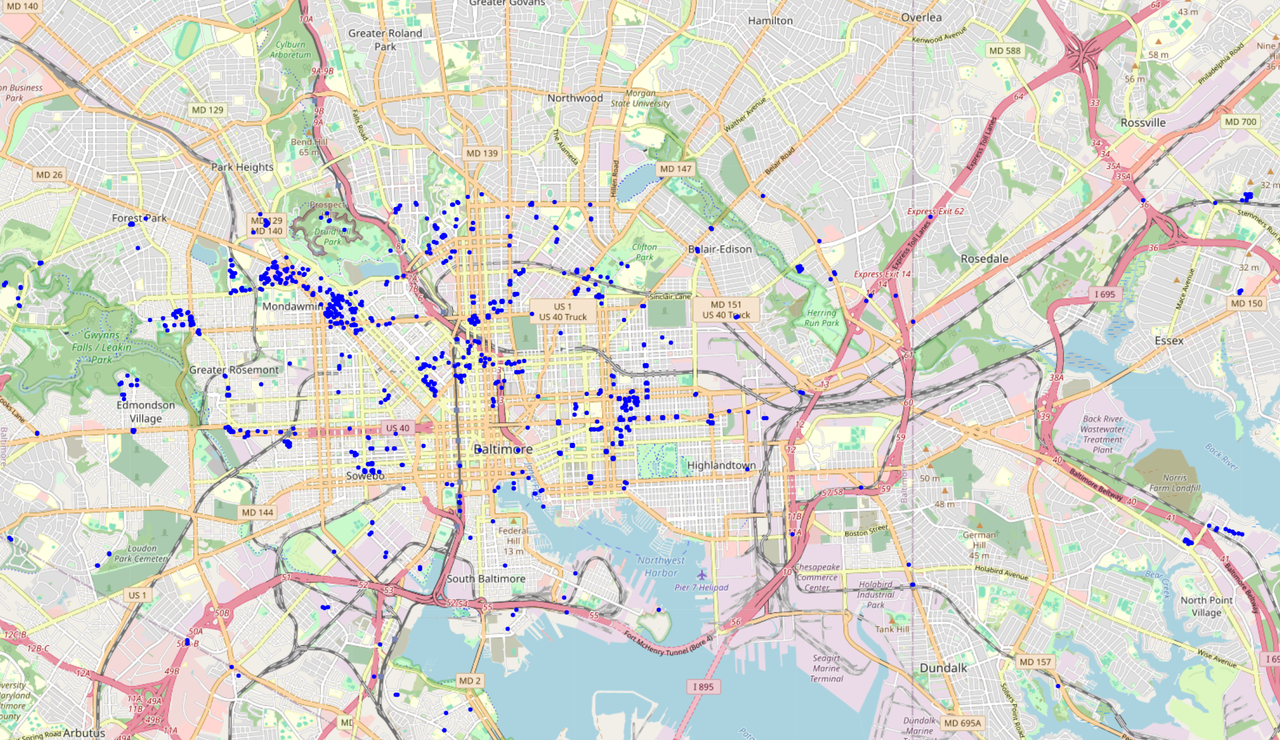
\includegraphics[width=0.65\textwidth]{figures/vis.png}
  \caption{Visualization of the Top 1000 Important Nodes}
  \label{fig:vis}
\end{figure}

\section{Problem 1: Application of the Transportation Network Model to the Collapse of the Francis Scott Key Bridge}

On March 26, 2024, a traffic accident caused the collapse of the Francis Scott Key Bridge, resulting in traffic paralysis. Based on the above - mentioned Baltimore transportation network model, our team analyzed the changes in node importance before and after the bridge collapse. We found that after the bridge collapse, the importance scores of adjacent road nodes (such as the I - 95 Tunnel and the I - 895 Tunnel) increased, and they became congestion hotspots on alternative routes. We calculated the node importance scores of the Baltimore transportation network before and after the bridge collapse respectively, and then drew a heatmap of the percentage increase in node importance after the bridge collapse. The results show that the importance of the I - 895 Tunnel increased most significantly, by about 63.701\%, followed by the I - 95 Tunnel, about 47.258\%, and the importance of the detour roads in the city also increased by an average of 10\% - 20\%. This also reveals the problems in the Baltimore urban transportation network: insufficient path redundancy and broken multi - mode connections.

\begin{figure}[H]
  \centering
  \subfigure[Before Collapse]{
  \begin{minipage}[t]{0.3\linewidth}
  \centering
  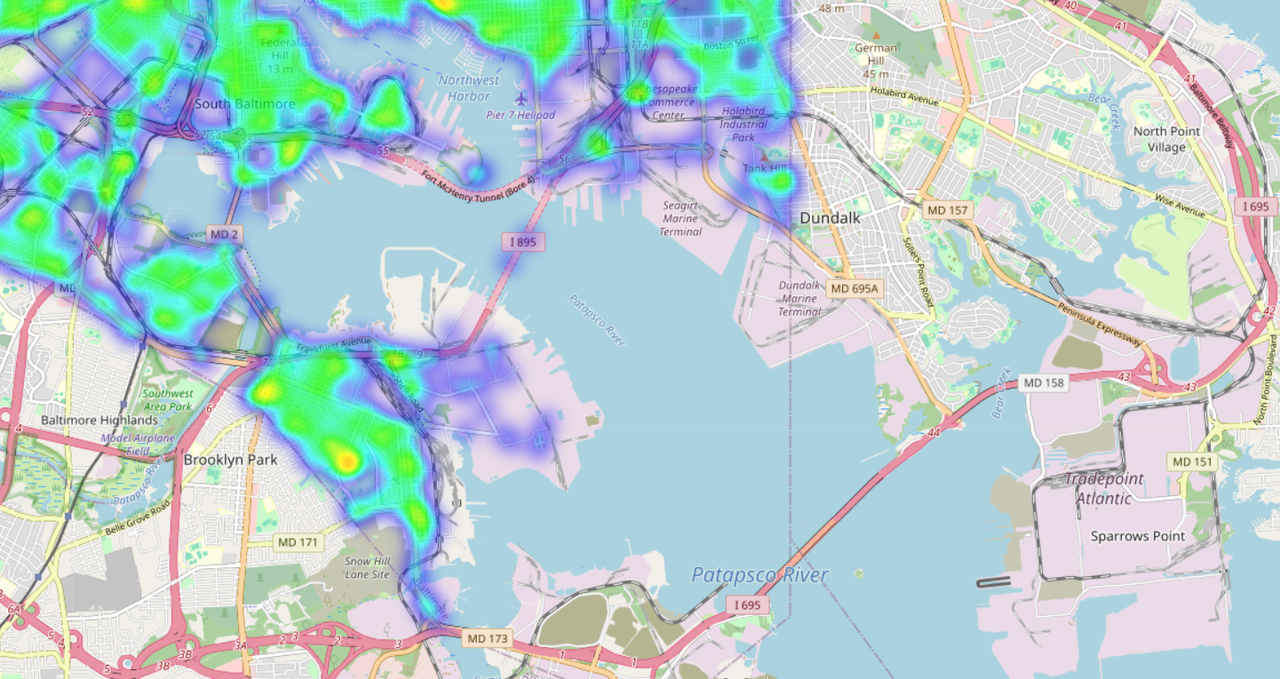
\includegraphics[width=\linewidth]{figures/heatmapbefore.png}
  \end{minipage}%
  % \label{fig:}%
  }%
  \subfigure[After Collapse]{
  \begin{minipage}[t]{0.7\linewidth}
  \centering
  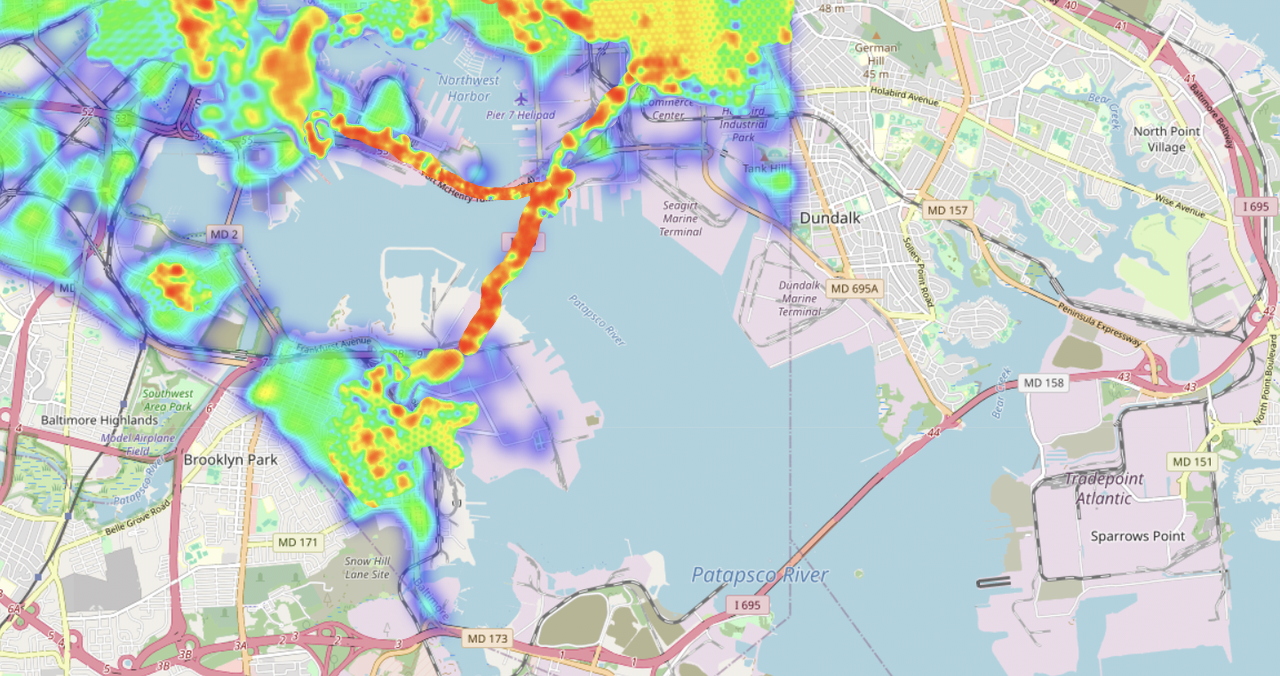
\includegraphics[width=\linewidth]{figures/heatmap.png}
  \end{minipage}%
  % \label{fig:}%
  }%
  \caption{Heatmap of Importance Increase}
  \label{fig:heatmap}
\end{figure}

Then, we calculated the increase in the importance of nodes in the Baltimore urban transportation network according to the $\alpha$ values of three different stakeholders: local residents, freight enterprises, and tourists. The results are shown in the following table. We found that before and after the collapse of the Francis Scott Key Bridge, the change in the importance of nodes in the Baltimore transportation network for local residents was minimal. This is because the activity scope of local residents is relatively fixed, and they generally do not go to the other side of the river. The change for tourists was slightly greater, as they are more likely to go to the other side than local residents. The change for freight enterprises was the highest, as they need to travel between the two sides frequently. In addition, it is worth noting that due to possible restrictions on passing vehicles in the I - 895 Tunnel and the I - 95 Tunnel, vehicles have to detour in the city, so the percentage increase in the importance of detour roads in the city is relatively high.

\begin{table}[H]
  \centering
  \caption{Importance Increase of Different Nodes for Stakeholder Groups}
  \begin{tabular}{lccc}
      \toprule
      Stakeholder Groups & I - 895 Tunnel & I - 95 Tunnel & Detours within the City \\
      \midrule
      Local Residents & 62.375\% & 46.046\% & 18.901\% \\
      Tourists & 64.528\% & 47.568\% & 15.679\% \\
      Freight Enterprises & 64.796\% & 48.586\% & 12.179\% \\
      \bottomrule
  \end{tabular}
\end{table}

\section{Problem 2: Application of the Transportation Network Model to Optimize Bus Routes}

\subsection{Feature Weight Analysis Based on PCA}

\subsubsection{Data Selection and Processing}

In the bus stop dataset \texttt{Bus\_Stops.csv}, we need to analyze the features of bus stops, determine the contribution weight of each feature to the clustering result, and perform clustering based on these weights. After screening, we removed some columns that were meaningless, had repeated meanings, or had single - valued data, and selected the following data indicators:
Categorical variables \texttt{Mode}, \texttt{Shelter}, and numerical variables \texttt{X}, \texttt{Y}, \texttt{Rider\_Total}, \texttt{Stop\_Rider}.

Since categorical features cannot be directly used in PCA\cite{Hotelling1933}, we first perform One - Hot encoding on them, and then determine the weight of each feature through PCA analysis. PCA is sensitive to the scale of data, so we need to standardize the numerical features.

\subsubsection{Principal Component Analysis}

The standardized data matrix is $\mathbf{X} \in \mathbb{R}^{n \times p}$, where $n$ is the number of samples and $p$ is the number of features. The formula for calculating the covariance matrix $\mathbf{C}$ is:

\begin{equation}
\mathbf{C} = \frac{1}{n - 1} \mathbf{X}^T \mathbf{X}
\end{equation}

Perform eigenvalue decomposition on the covariance matrix $\mathbf{C}$:
\begin{equation}
\mathbf{C} = \mathbf{V} \mathbf{\Lambda} \mathbf{V}^T
\end{equation}
where $\mathbf{V}$ is the matrix of eigenvectors and $\mathbf{\Lambda}$ is the diagonal matrix of eigenvalues.

The principal components $\mathbf{P}$ are the projections of the original data in the direction of the eigenvectors:
\begin{equation}
\mathbf{P} = \mathbf{X} \mathbf{V}
\end{equation}

The variance contribution rate of each principal component is:
\begin{equation}
\text{Explained Variance Ratio}_i = \frac{\lambda_i}{\sum_{j = 1}^p \lambda_j}
\end{equation}
where $\lambda_i$ is the $i$-th eigenvalue.

\subsubsection{Feature Weight Calculation}

For categorical features, such as \texttt{Mode} and \texttt{Shelter}, we use One - Hot encoding to convert them into binary vectors. Suppose the categorical feature $\mathbf{C}$ has $k$ values, then the feature matrix after One - Hot encoding is:
\begin{equation}
\mathbf{C}_{\text{encoded}} \in \mathbb{R}^{n \times k}
\end{equation}

Combine the standardized numerical features $\mathbf{X}_{\text{scaled}}$ and the One - Hot encoded categorical features $\mathbf{C}_{\text{encoded}}$:
\begin{equation}
\mathbf{X}_{\text{processed}} = [\mathbf{X}_{\text{scaled}}, \mathbf{C}_{\text{encoded}}]
\end{equation}

Perform PCA analysis on the combined data $\mathbf{X}_{\text{processed}}$ to obtain the variance contribution rate $\text{Explained Variance Ratio}_i$ of each principal component. Combine the variance contributions of the One - Hot encoded features back to the original categories. Suppose the variance contributions corresponding to the One - Hot encoded columns of the original categorical feature $\mathbf{C}$ are $\text{Explained Variance Ratio}_j$, then the weight of the original category is:
\begin{equation}
\text{Weight}_i = \sum_{j \in \text{Category}_i} \text{Explained Variance Ratio}_j
\end{equation}

Normalize the weights so that their sum is 1:
\begin{equation}
\text{Normalized Weight}_i = \frac{\text{Weight}_i}{\sum_{j = 1}^p \text{Weight}_j}
\end{equation}

So far, we have calculated the weights of the shown data, and the results are as follows:

\begin{table}[H]
  \centering
  \caption{Data Meanings and Their Weights}
  \label{tab:data_weights}
  \begin{tabular}{@{}lcc@{}}
      \toprule
      \textbf{Data Meaning} & \textbf{Variable} & \textbf{Weight} \\
      \midrule
      Total Number of Riders & \texttt{Rider\_Tota} & 0.62830 \\
      Total Cumulative Number of Riders at Stops & \texttt{Stop\_Rider} & 0.21777 \\
      Transportation Mode Type (e.g., bus) & \texttt{Mode} & 0.03646 \\
      Whether There is a Passenger Shelter & \texttt{Shelter} & 0.00093 \\
      Service Type of Bus & \texttt{Routes\_Ser} & 0.11650 \\
      \bottomrule
  \end{tabular}
\end{table}

\subsection{Bus Stop Clustering Based on K-Prototypes}

The K-Prototypes algorithm\cite{Huang1998} is a clustering method capable of handling both numerical and categorical data simultaneously. Our dataset contains both numerical and categorical features, which fully meets the requirements of the K - Prototypes algorithm. In addition, as calculated in Table \ref{tab:data_weights} through PCA analysis, we have obtained the weight contributions of each feature, and these weights will be used to optimize the clustering process.

Unlike the K-means algorithm, the K-Prototypes algorithm can calculate the similarity of numerical types not only through the Euclidean distance but also calculate the similarity of categorical types through the Hamming distance.

We performed clustering on the bus stop data in Baltimore. After selecting different values of $k$ multiple times, we found that the effect was relatively ideal when $k = 5$. The visualization result of the clustering is shown in the figure below:

\begin{figure}[H]
  \centering
  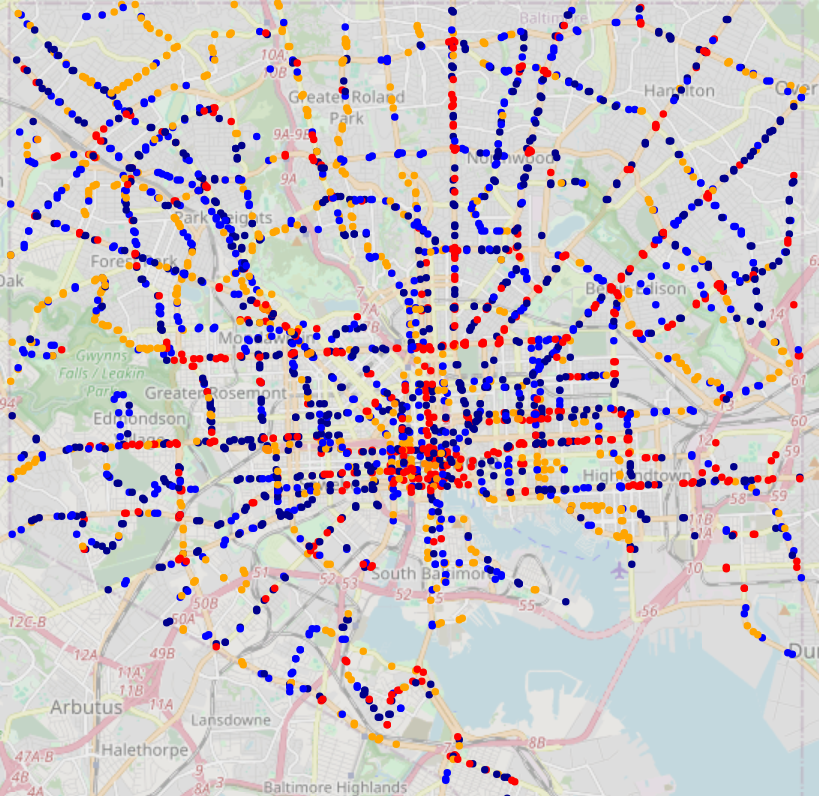
\includegraphics[width=0.7\textwidth]{figures/cluster.png}
  \caption{Visualization of Bus Stop Clustering}
  \label{fig:cluster}
\end{figure}

By observing the clustering result graph, we noticed that the stations with the highest importance are largely concentrated in the city center, distributed along busy traffic routes. While the stations with low importance are mostly concentrated in areas far from the city center, distributed along traffic routes with low human flow. Therefore, we consider selecting the area where the stations with high importance are concentrated for further analysis.

\subsection{Bus Route Optimization Based on Clustering Results}

We extracted one part of the clustering results for analysis and attempted to plan the addition of bus routes for this area. To this end, we calculated the corresponding score for each station and added bus routes in places with high scores. Besides the node weights in Section 4, for bus routes, we should also pay attention to the influence of passenger flow and the number of bus routes on the score: the larger the passenger flow, the more bus routes should be added; and the fewer the number of bus routes, the more bus routes should be added. The specific formula for calculating the score is as follows\footnote{According to Assumption 3, the passenger flow is \texttt{Rider\_Tota}, and the number of bus routes is the length of the \texttt{Routes\_Ser} list.}:

\begin{equation}
score=\dfrac{\text{Passenger Flow}\times \text{Average Importance of Nodes on Both Sides of the Station}}{\text{Number of Bus Routes}}
\end{equation}

Due to the geographical distribution of multiple hospitals and universities, we believe that adding bus routes to the red - line part is the optimal choice, as shown in Figure \ref{fig:busroute}.

\begin{figure}[H]
  \centering
  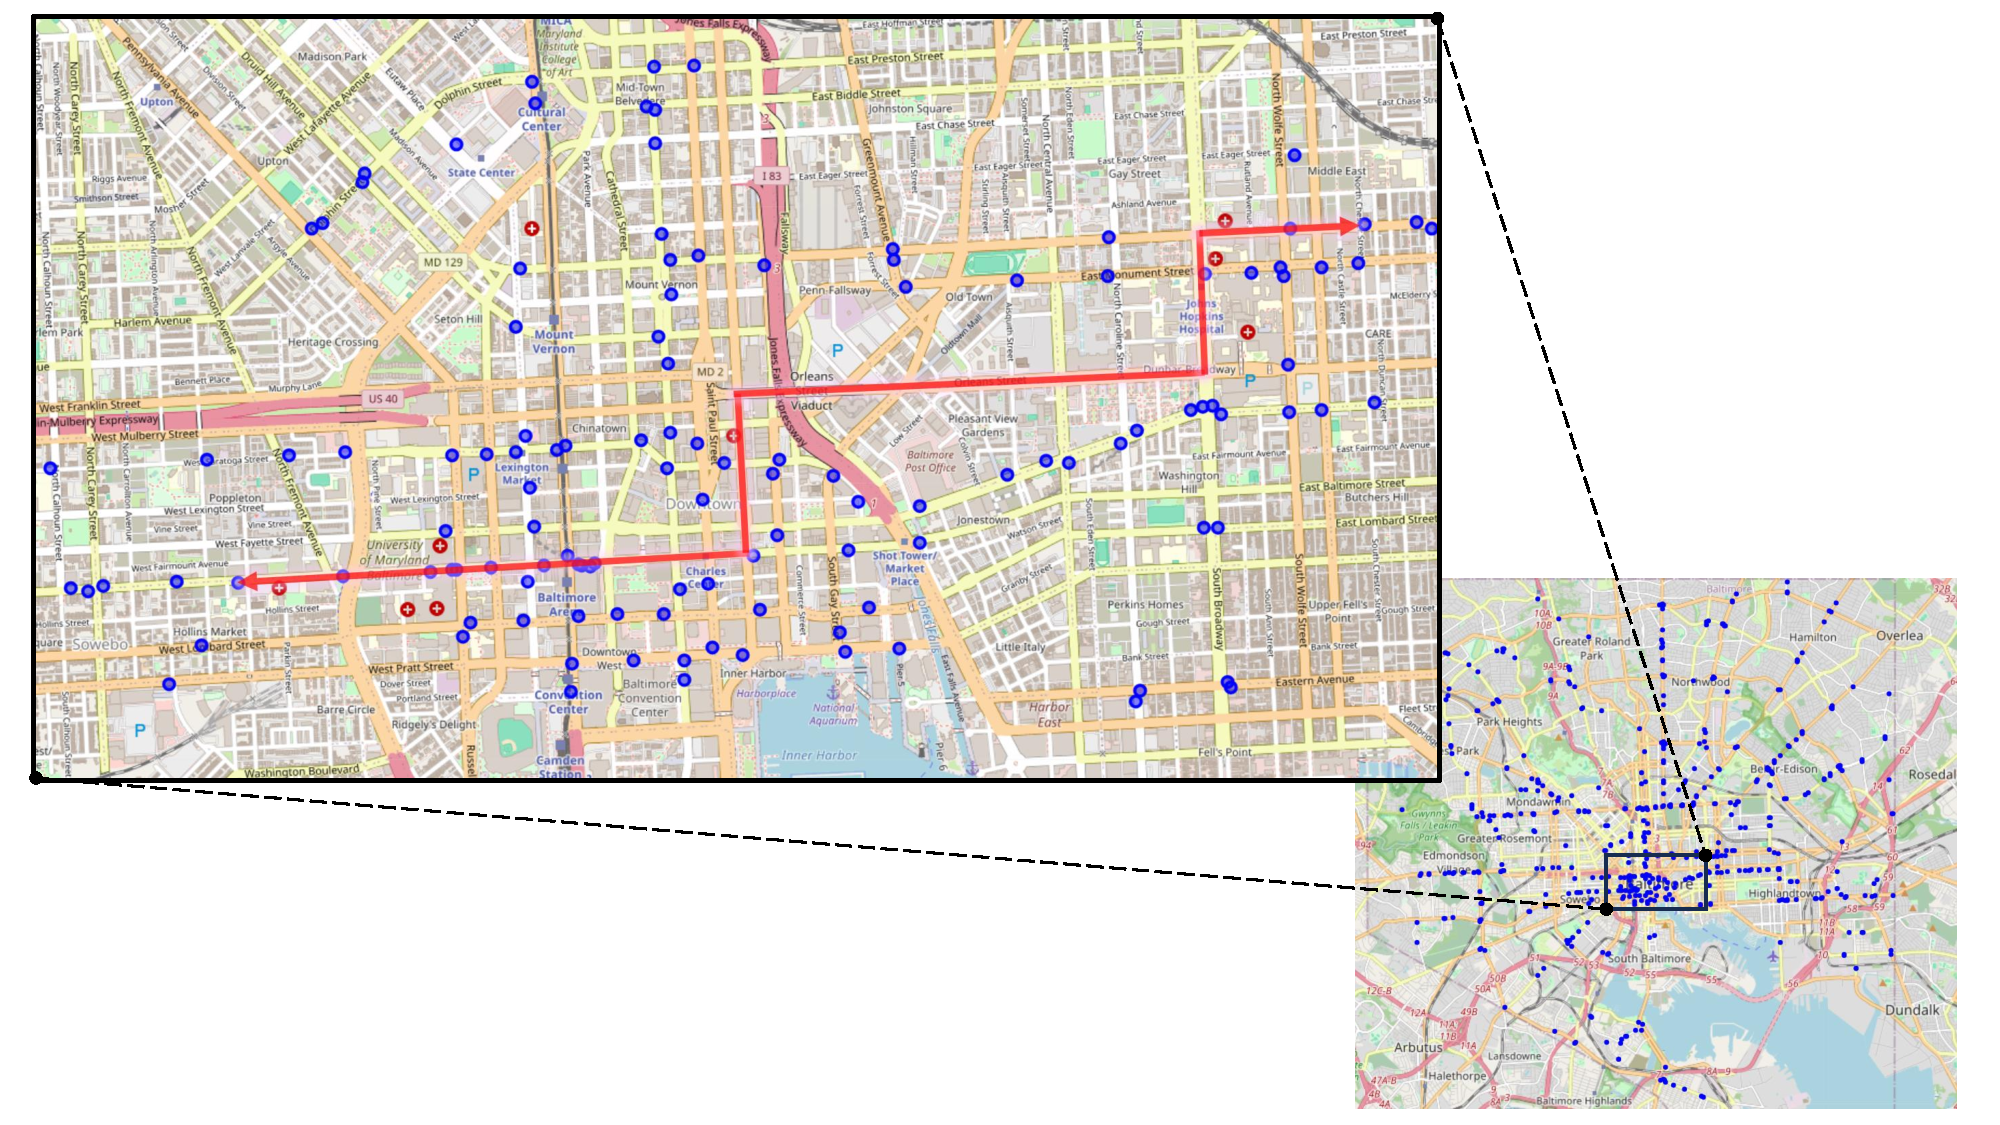
\includegraphics[width=\textwidth]{figures/busroute.pdf}
  \caption{Bus Route Optimization Plan}
  \label{fig:busroute}
\end{figure}

\subsection{Impact on Stakeholders in the Surrounding Areas}

After adding new bus routes at the places marked with the red line on the map, it has greatly facilitated the daily travel of the surrounding residents and significantly improved the travel experience of tourists. At the same time, it has reduced the willingness of residents such as university students to travel by car, providing a more convenient logistics channel for freight companies. This improvement not only strengthens the connection of the transportation network within the region but also promotes the local economic development, enabling residents, tourists, and enterprises to benefit from it.

\section{Problem 3: Congestion Management Strategy for the Baltimore Transportation Network}

\subsection{Traffic Hazards in Baltimore}

Traffic network congestion in the city has always been a safety hazard in Baltimore. It may not only increase the probability of traffic accidents but also lead to an increase in the crime rate in areas with inconvenient transportation due to the difficulty of the police arriving quickly. In addition, stampede accidents may occur in densely populated areas, and crimes such as theft and robbery are also likely to happen. Therefore, our team has designed a congestion management strategy for the Baltimore transportation network. By analogy with the congestion control algorithm in the field of computer networks, we adjust the signal light cycle and the number of traffic police dynamically in stages.

\subsection{Exponential Model of Traffic Congestion and Congestion Management Strategy}


According to the classical LWR model to describe the traffic density $\rho(x,t)$, we have:
\begin{equation}
\frac{\partial \rho}{\partial t} + \frac{\partial}{\partial x} \left( \rho v(\rho) \right) = 0\Rightarrow v(\rho) = v_{\text{free}} \left( 1 - \frac{\rho}{\rho_{\text{max}}} \right)
\end{equation}
where $\rho(x,t)$ is the traffic flow density, $v(\rho)$ is the traffic flow speed, and $\rho_{\text{max}}$ is the road - carrying capacity.

Considering that the importance of the node $w_i$ weakens the local traffic capacity:
\begin{equation}
\rho_{\text{max},i} = \rho_{\text{base}} \cdot \left( 1 - \alpha w_i \right)
\end{equation}

In the local road section (near node $i$), ignoring the spatial derivative term, the LWR equation degenerates into the Logistic equation:
\begin{equation}
\frac{d\rho_i}{dt}=k_i\rho_i\left(1-\frac{\rho_i}{\rho_{\max,i}}\right)
\end{equation}

Considering that the higher the importance of the node, the faster the congestion may spread. Define the modified growth rate:
\begin{equation}
k_i=k_{\mathrm{base}}\cdot(1+\beta w_i)
\end{equation}

Substituting it into the above equation, we get:
\begin{equation}
\frac{d\rho_i}{dt} = k_{\text{base}} (1 + \beta w_i) \rho_i \left( 1 - \frac{\rho_i}{\rho_{\text{base}} (1 - \alpha w_i)} \right)
\end{equation}

Solving the above equation by the method of separation of variables:
\begin{equation}
\rho_i(t) = \frac{\rho_{\text{max},i}}{1 + e^{-k_{\text{base}} (1 + \beta w_i) t} \cdot \left( \frac{\rho_{\text{max},i}}{\rho_{i,0}} - 1 \right)}
\end{equation}

When $\rho_i \ll \rho_{\text{max},i}$:
\begin{equation}
\rho_i(t) \approx \rho_{i,0} \cdot e^{k_{\text{base}} (1 + \beta w_i) t}
\end{equation}

In the early stage of congestion, the degree of congestion will increase exponentially with time. After reaching a certain critical value, the growth of the congestion degree begins to slow down, which is very similar to the congestion control in the TCP protocol \cite{Jacobson1988}. Therefore, we propose the following congestion management strategies:

\begin{itemize}
    \item Stage 1: In the initial stage of congestion, the degree of congestion increases exponentially with time. At this time, the signal light cycle should be adjusted at major intersections, and the number of traffic police should be increased rapidly.
    \item Stage 2: In the middle and late stages of congestion, the growth of the congestion degree slows down, and so does the number of additional traffic police.
    \item Stage 3: After the congestion ends, the signal light cycle and the number of traffic police return to normal levels.
\end{itemize}

\begin{figure}[H]
  \centering
  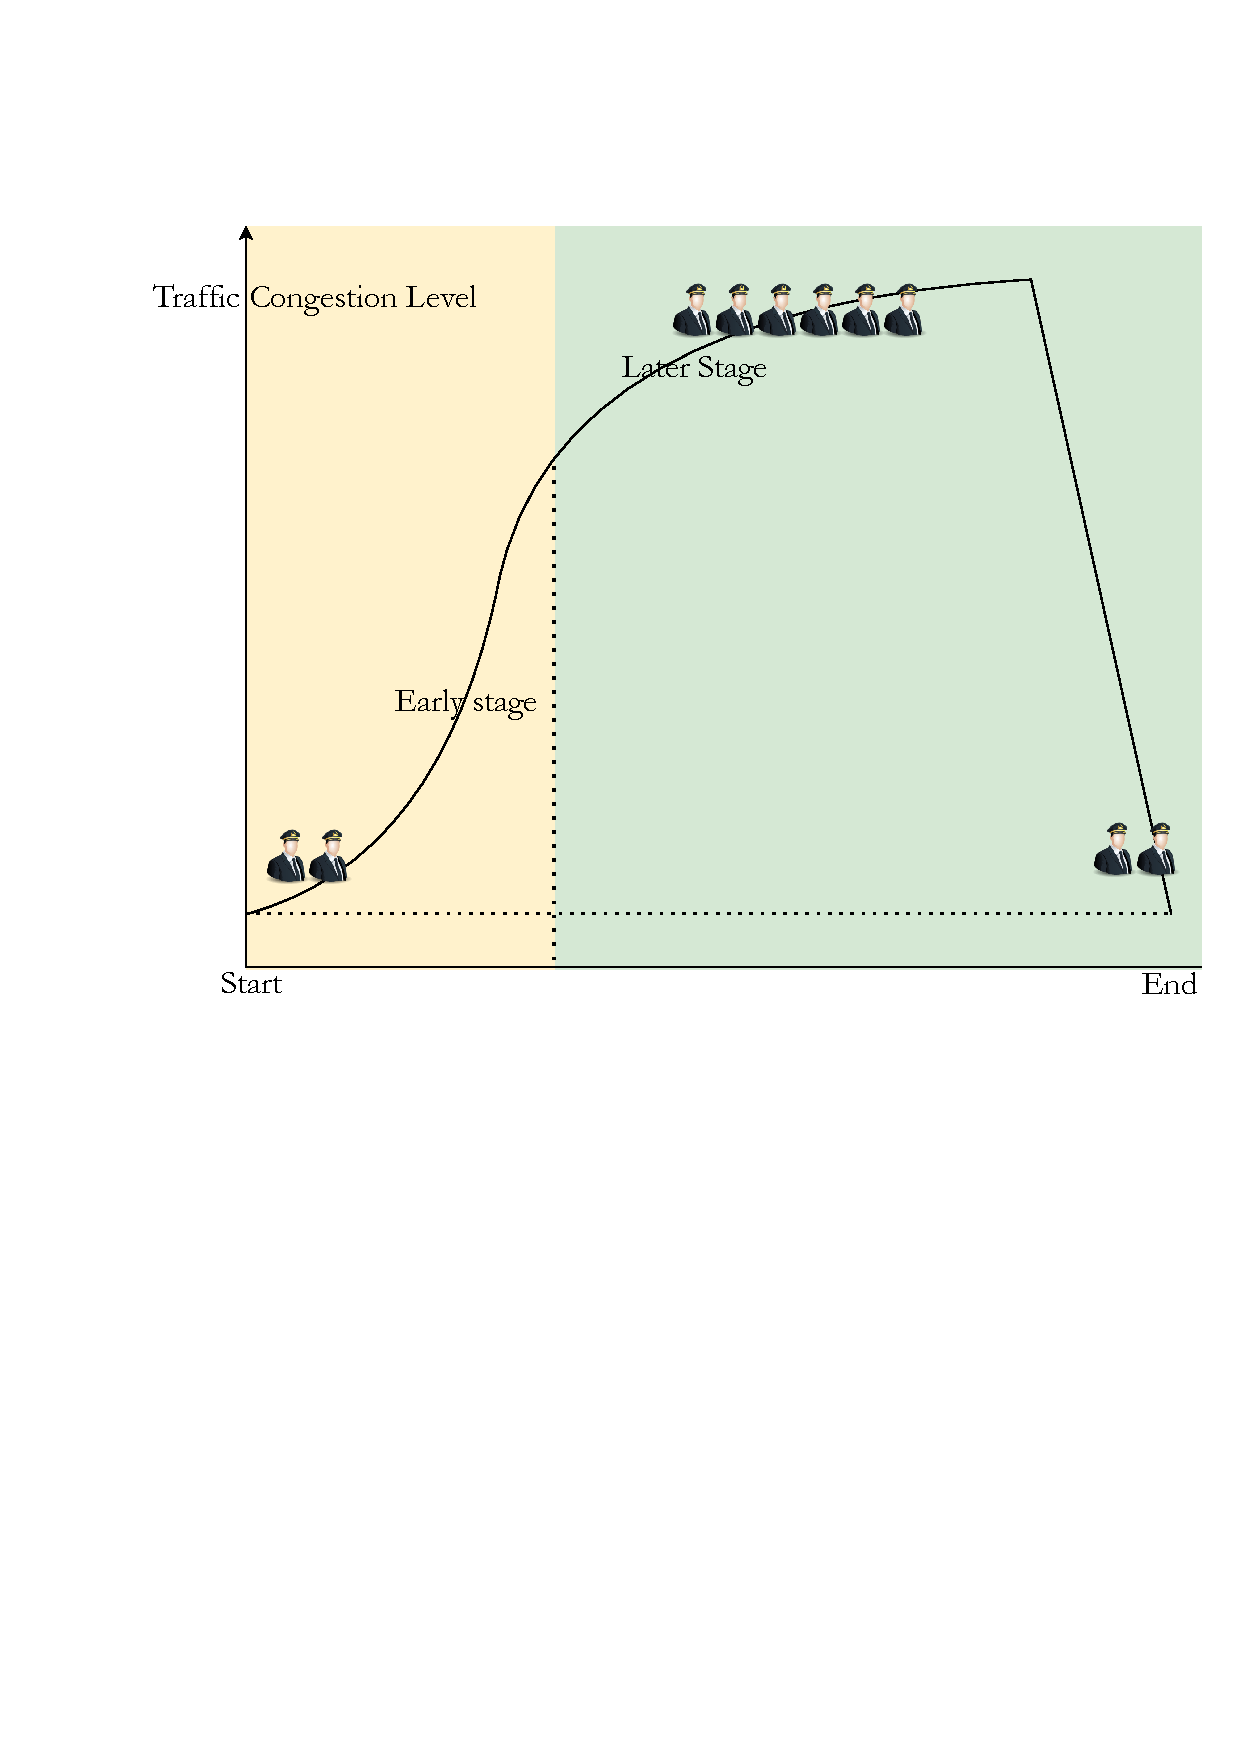
\includegraphics[width=0.7\textwidth]{figures/3stage.pdf}
  \caption{Schematic Diagram of Congestion Management Strategy}
  \label{fig:3stage}
\end{figure}

\subsection{Impact of Traffic Congestion Management Strategy on the Interests of All Parties}

\begin{table}[H]
  \centering
  \caption{Stakeholders and Their Concerns}
  \label{tab:stakeholder_concerns}
  \begin{tabularx}{\textwidth}{@{}lXX@{}} 
      \toprule
      \textbf{Stakeholders} & \textbf{Convenience of Travel} & \textbf{Safety of Travel} \\
      \midrule
      Local Residents & Shorter travel time, more travel options, and an improved quality of life & Fewer traffic accidents and the rapid arrival of police forces \\
      Tourists & Enhanced travel convenience and an improved tourism experience & Reduced stampede accidents and a lower crime rate \\
      Freight Enterprises & Higher transportation efficiency and lower transportation costs & Fewer traffic accidents and improved cargo safety \\
      \bottomrule
  \end{tabularx}
\end{table}

We summarize the impact of traffic congestion management on various stakeholders in Baltimore as shown in Table \ref{tab:stakeholder_concerns}. The traffic congestion management strategy in Baltimore not only facilitates the travel of local residents, tourists, and freight enterprises but also has a positive impact on the safety of the city. By dynamically adjusting the signal light cycle and increasing the number of traffic police, traffic congestion can be effectively reduced, travel efficiency and safety can be improved, the quality of life of residents and the tourism experience of tourists can be enhanced, the transportation costs of freight enterprises can be lowered, and the economic development of the city can be promoted.


\section{Sensitivity Analysis}

We increased and decreased the $\alpha$ values calculated in Section 4.4 by 5\% respectively, and calculated the mean squared errors between the results after the increase or decrease and the original $\alpha$ values. The results are shown in Table \ref{tab:alpha_mse}:

\begin{table}[H]
    \centering
    \caption{Mean Squared Errors of $\alpha$ Values after Perturbation}
    \label{tab:alpha_mse}
    \begin{tabular}{@{}lcc@{}}
        \toprule
        & \textbf{$\alpha$ Value} & \textbf{Mean Squared Error} \\
        \midrule
        Original Value & 0.32534 & \(\varnothing\) \\
        Increased by 5\% & 0.341607 & 14.209293 \\
        Decreased by 5\% & 0.309073 & 8.608151 \\
        \bottomrule
    \end{tabular}
\end{table}

The results show that after making small perturbations to the parameter $\alpha$, the resulting differences are within an acceptable range, which proves the robustness of our model.

\section{Advantages and Disadvantages}
\subsection{Advantages}
\begin{enumerate}
    \item Our improved K-Shell decomposition algorithm with node weights and edge weights can comprehensively construct the traffic network graph model of the city from aspects such as the actual traffic situation and the topological structure of the traffic network, which is relatively comprehensive.
    \item By introducing proportional coefficients for node weights and edge weights, the influence of various stakeholders is analyzed and deeply considered.
    \item When clustering with the K-Prototypes algorithm, the weights of each type are determined by the PCA algorithm, which is relatively accurate.
\end{enumerate}

\subsection{Disadvantages and Improvements}
\subsubsection{Disadvantages}
\begin{enumerate}
    \item When calculating edge weights, the AADT value of each road is required. However, not every road has a bus stop. If the shortest - distance algorithm is directly used to fill the data, the time complexity is too high.
    \item The k - means clustering algorithm calculates similarity based on Euclidean distance and cannot handle categorical data.
\end{enumerate}

\subsubsection{Improvements}
\begin{enumerate}
    \item Similar to the watershed algorithm in the field of computer vision\cite{Vincent1991}, our team has constructed a fast algorithm for filling the missing AADT values. See section \ref{sec:improvedKshell} This algorithm can complete the filling task with almost linear time complexity, meeting the filling requirements for large - scale graph network data.
    \item K - Prototype is an extended version of K - means, which can handle both numerical and categorical data and can well complete the clustering task in Section 6.2.
\end{enumerate}

% \addcontentsline{toc}{section}{Letter} % Add section to the table of contents
% 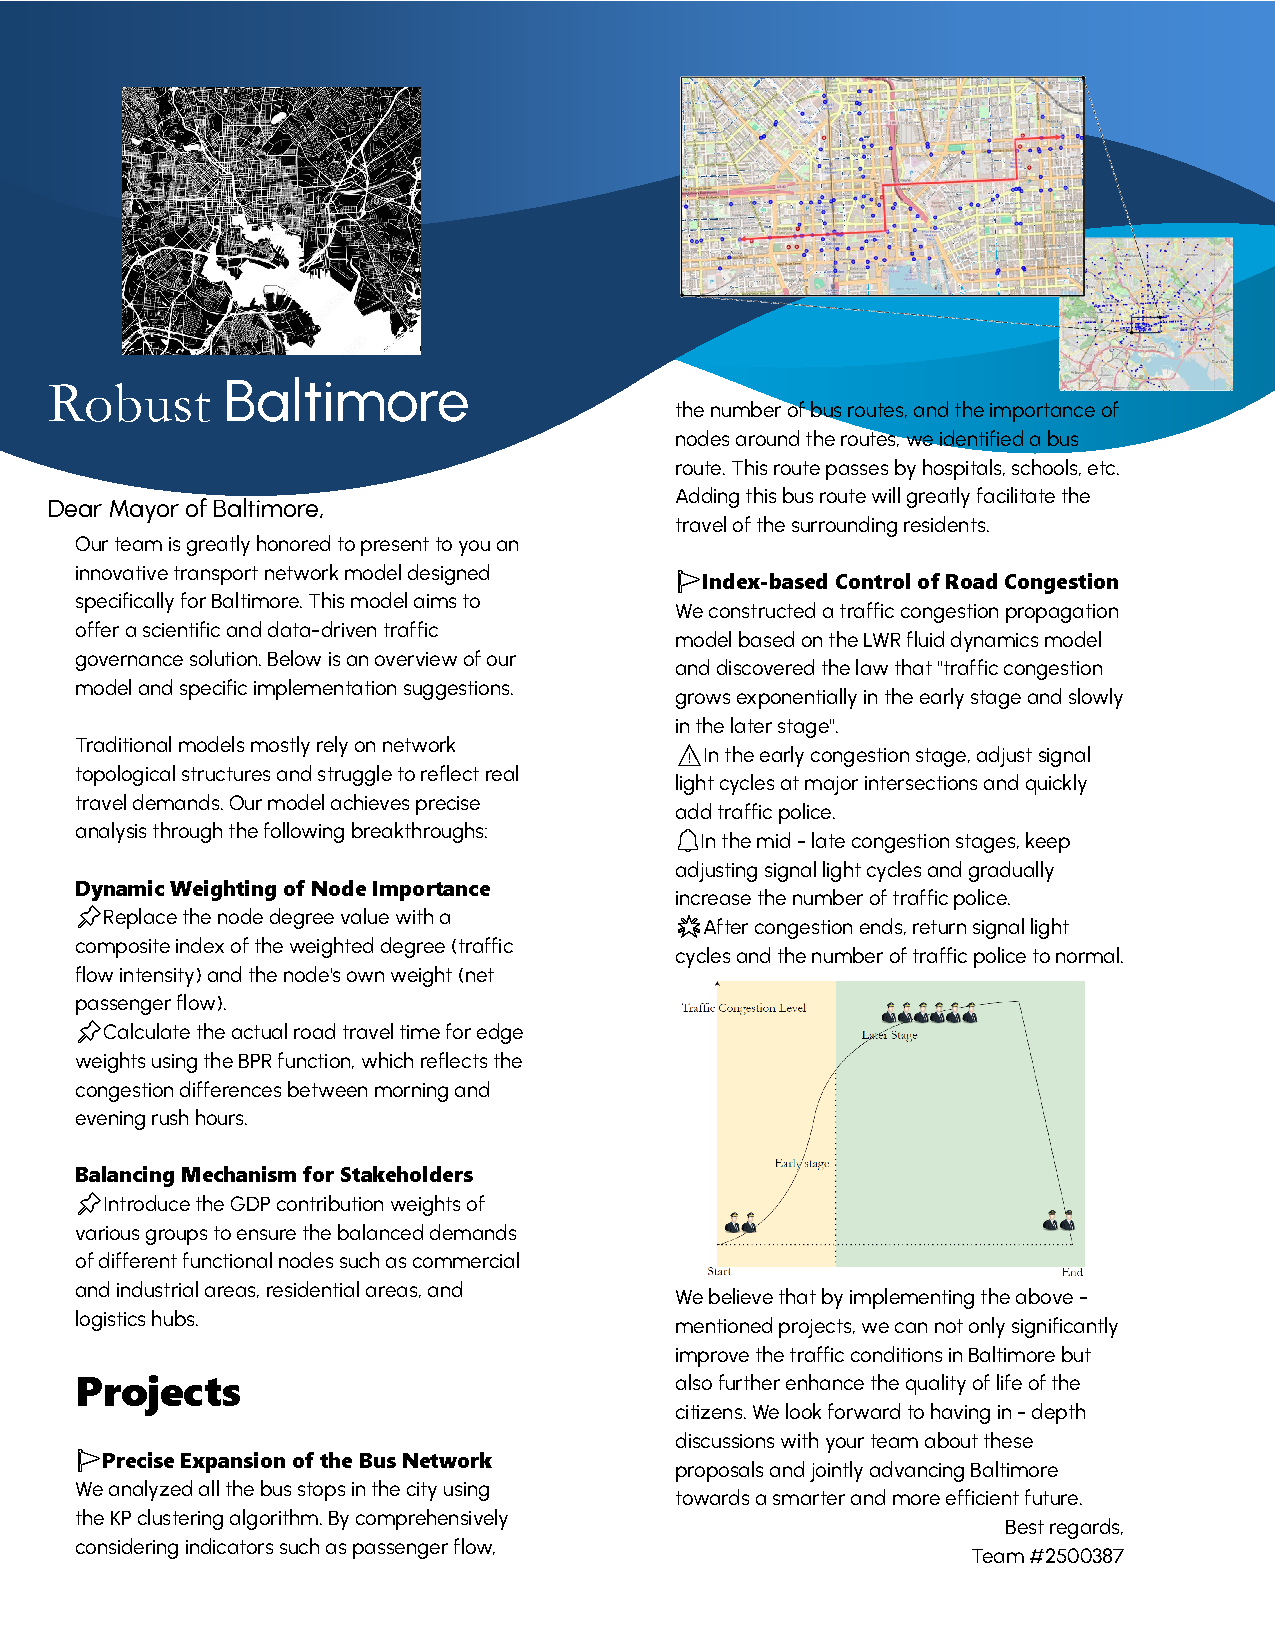
\includepdf[pages=-]{figures/letter.pdf}
\addcontentsline{toc}{section}{Letter} % 将 section 添加到目录中
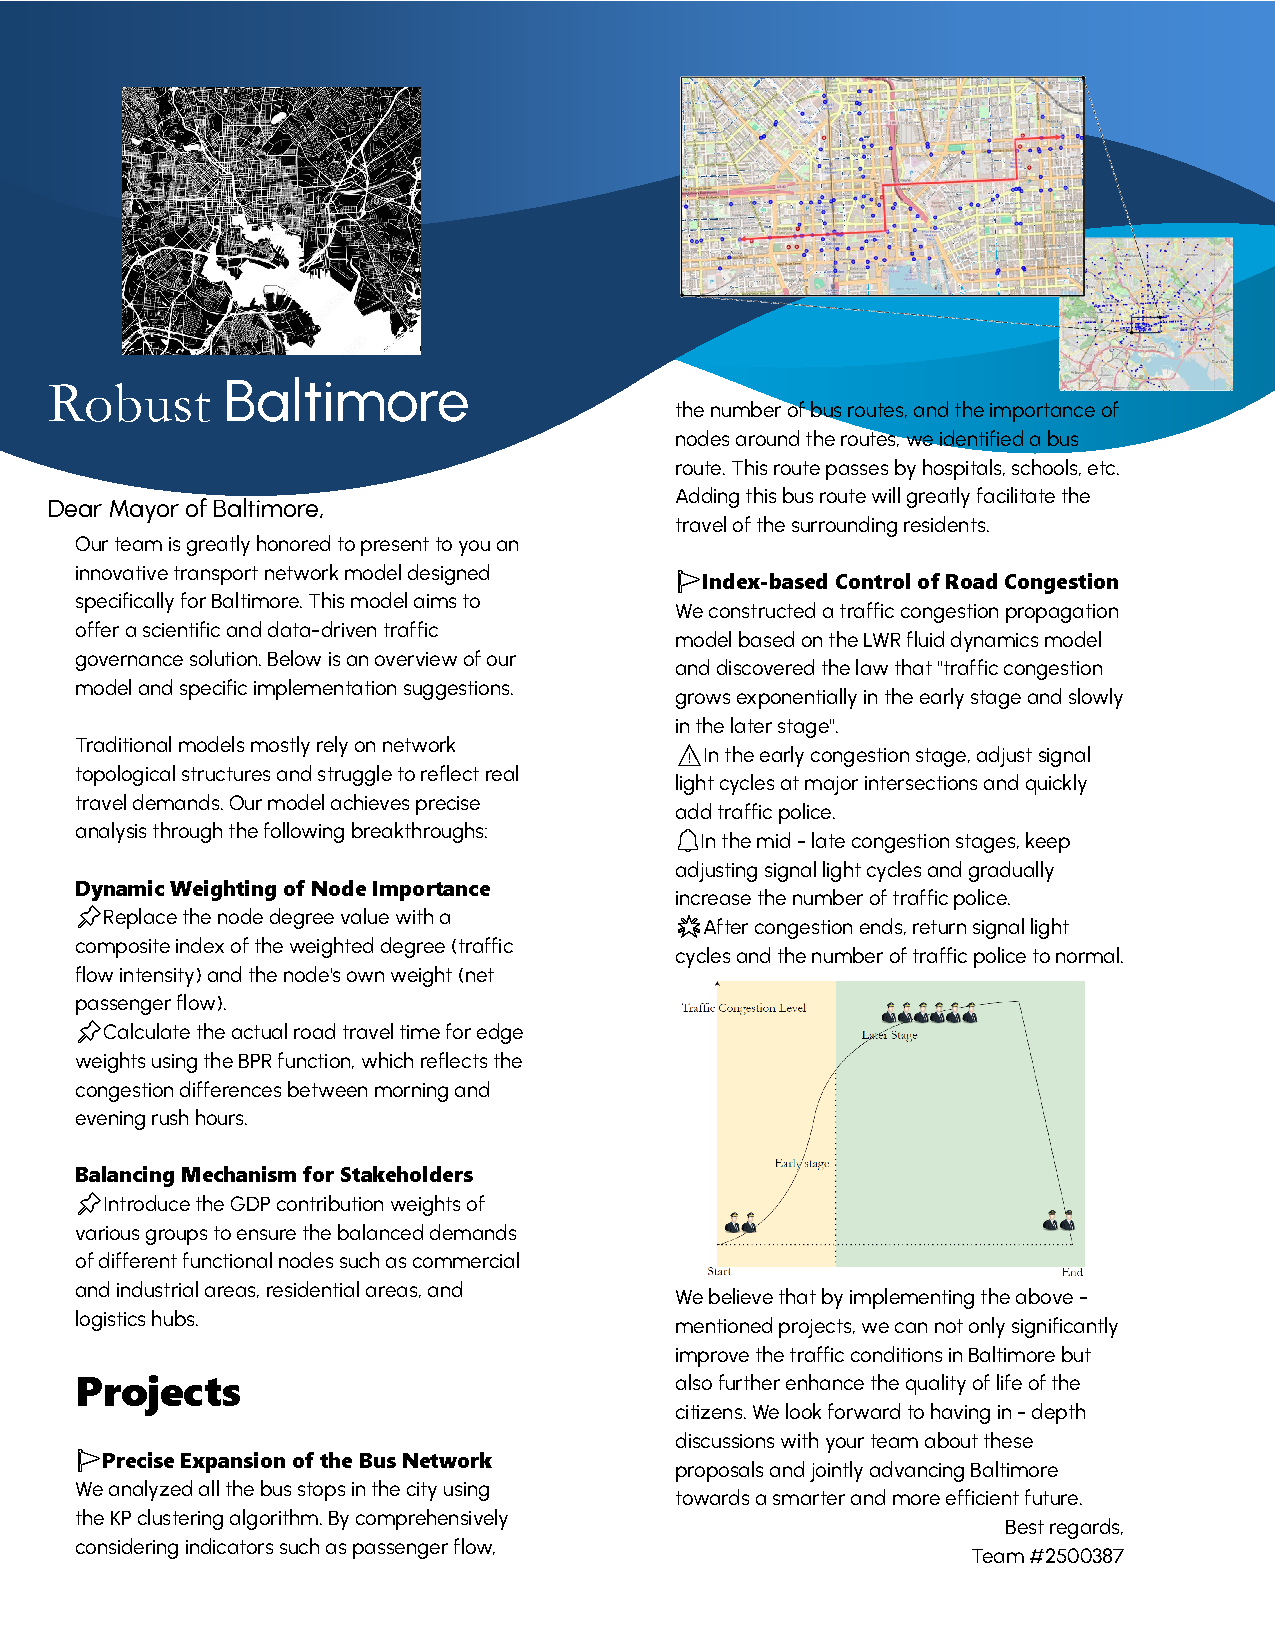
\includepdf[pages=-]{figures/letter.pdf}


\newpage
\addcontentsline{toc}{section}{Reference} 
\bibliographystyle{unsrt}
\bibliography{ref}
\section{Appendix}

\subsection{Stakeholders and Their GDP Data Sources}
\label{sec:source}
\begin{table}[H]
  \centering
  \begin{tabularx}{\textwidth}{lX}
      \toprule
      Stakeholders & GDP Data Sources \\
      \midrule
      Local Residents & \url{https://fred.stlouisfed.org/series/PCPI24510}, \url{https://fred.stlouisfed.org/series/MDBALT5POP} \\
      Freight Enterprises & \url{https://fred.stlouisfed.org/series/GDPALL24510} \\
      Tourists & \url{https://baltimore.org/about-us/} \\
      \bottomrule
  \end{tabularx}
\end{table}

\subsection{Improved K-Shell algorithm based on node weights and edge weights}

\begin{lstlisting}
def weighted_k_shell_with_node_weights(graph, node_weights):
    weighted_degree = {node: sum(data['weight'] for _, data in graph[node].items()) for node in graph.nodes}
    k_shell = {}
    k = 0
    alpha = 0.32534
    while graph.number_of_nodes() > 0:
        composite_score = {node: alpha * weighted_degree[node] + (1 - alpha) * node_weights[node] for node in graph.nodes}
        min_composite_score = min(composite_score.values())
        to_remove = [node for node, score in composite_score.items() if score <= min_composite_score]
        for node in to_remove:
            k_shell[node] = k
        for node in to_remove:
            neighbors = list(graph.neighbors(node))
            graph.remove_node(node)
            del weighted_degree[node]
            for neighbor in neighbors:
                if neighbor in graph.nodes:
                    if neighbor in graph and node in graph[neighbor]:
                        weighted_degree[neighbor] -= graph[neighbor][node].get('weight', 0)
        k += 1
    return k_shell
\end{lstlisting}

\end{document}

